% !TeX program = lualatex
% !TeX encoding = UTF-8
% !TeX spellcheck = fr_FR

\documentclass[10pt, french,aspectratio=43]{beamer}
\setbeamertemplate{navigation symbols}{\insertframenumber}
\setbeamertemplate{footline}{$\quad$ \insertframenumber / \inserttotalframenumber}
\usepackage{polyglossia}
\setdefaultlanguage{french}
\usepackage{fontspec}
\defaultfontfeatures{Ligatures={Common ,TeX}}
\usepackage{hyperref}
\usepackage{mathtools , amssymb}
\usepackage{xcolor}
\usepackage{graphicx}
\usepackage{geometry}
\usepackage{stmaryrd}
\usepackage{subcaption}
\usepackage{multicol}
\captionsetup[sub]{subrefformat=brace}
\usepackage{dsfont}


\definecolor{airforceblue}{rgb}{0.36, 0.54, 0.66}
\definecolor{charcoal}{rgb}{0.21, 0.27, 0.31}
\definecolor{ube}{rgb}{0.53, 0.47, 0.76}
\definecolor{violet}{rgb}{0.2, 0.2, 0.6}

\usepackage[procnames]{listings}
\lstset{language=Python ,
mathescape=true,
frame=trBL,
numbers=none,
lineskip=0.01mm,
backgroundcolor=\color{white},
basicstyle=\scriptsize,
keywordstyle=\color{airforceblue},
commentstyle=\color{ube},
stringstyle=\color{red},
identifierstyle=\color{black},
breaklines=true,
inputpath={C:/Users/Adrien Dubois/Desktop/TIPE/2-Code/}}
\graphicspath{{C:/Users/Adrien Dubois/Desktop/TIPE/2-Code/images/}}


\usetheme{Marburg}
\title{Application de méthodes de recherche d'isomorphismes de graphes à la comparaison des structures de protéines}
\author{Adrien Dubois - N°candidat : 51771}
\date{\today}

\begin{document}
\part{Présentation}
\maketitle

\begin{frame}{Plan}
\tableofcontents
\end{frame}

\section{Contexte, données à traiter et objectif}
\begin{frame}{Contexte, données à traiter et objectif}
Compétition Casp
\begin{center}
\footnotesize
\begin{tabular}{ccc}
    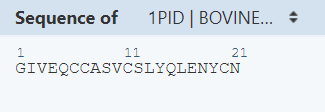
\includegraphics[width=3cm]{sequence_insuline_bovine}
    & 
    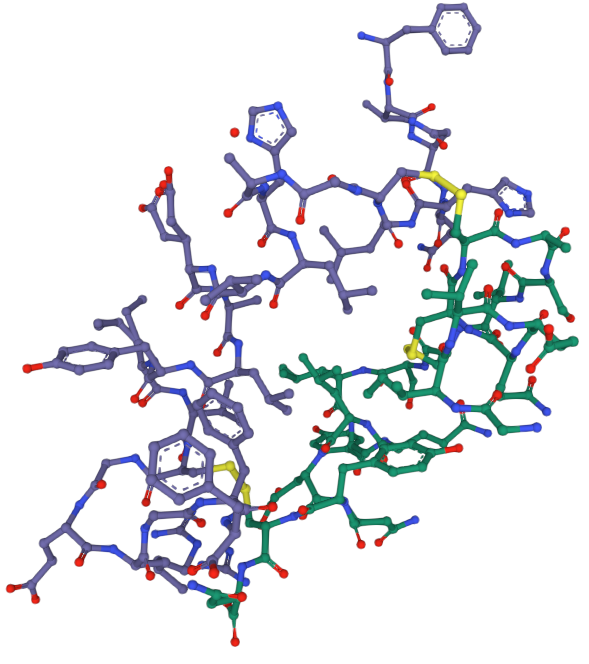
\includegraphics[width=2cm]{structure_insuline_bovine}
    &
    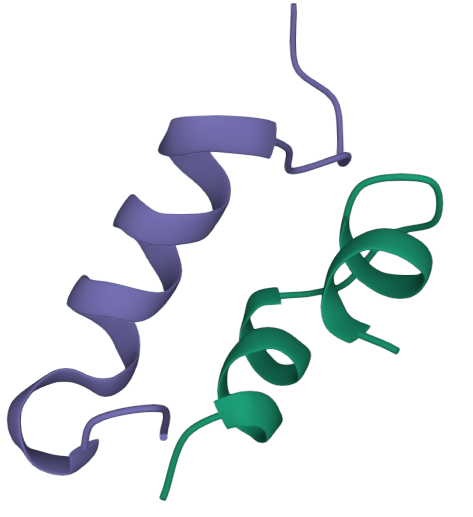
\includegraphics[width=2cm]{cartoon_insuline_bovine} \\
    \textit{Séquence} & \textit{Structure} & \textit{Représentation simplifiée}
\end{tabular}
\newline \newline \underline{ex} : protéine d'insuline bovine 
\footnote{source : Protein Data Bank, https://www.rcsb.org/3d-view/1B0Q}
\end{center}
\small
\underline{Objectif} : proposer une méthode de comparaison de structures
\end{frame}

\section{Comparaison de branches sans ramifications}
\begin{frame}{Format PDB et représentation}
    \footnotesize
    \begin{figure}[!htb]
        \centering
        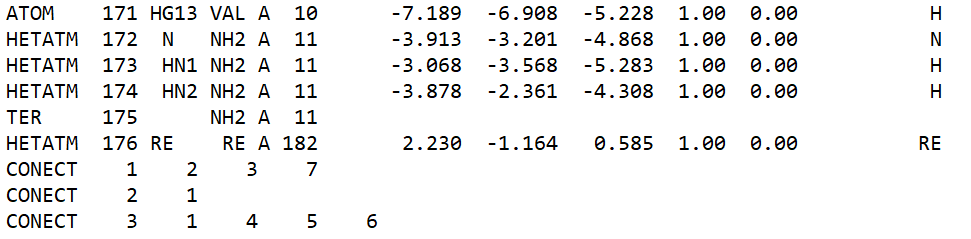
\includegraphics[width=9cm]{lignes_pdb}
        \caption{\label{PDB_tuto:http://acces.ens-lyon.fr/}Lignes d'un fichier PDB \footnote{source : http://acces.ens-lyon.fr/}}
    \end{figure}
    \begin{minipage}{0.45\textwidth}%
    \begin{center}
        \underline{Données}
    \end{center}
    \begin{tabular}{ccc}
    position des atomes & $\rightarrow$ & OK \\
    type des atomes & $\rightarrow$ & OK \\
    liaisons & $\rightarrow$ & moyennes
    \end{tabular}
    \end{minipage}%
    \hfill
    \begin{minipage}{0.45\textwidth}%
    \begin{figure}[!htb]
        \centering
        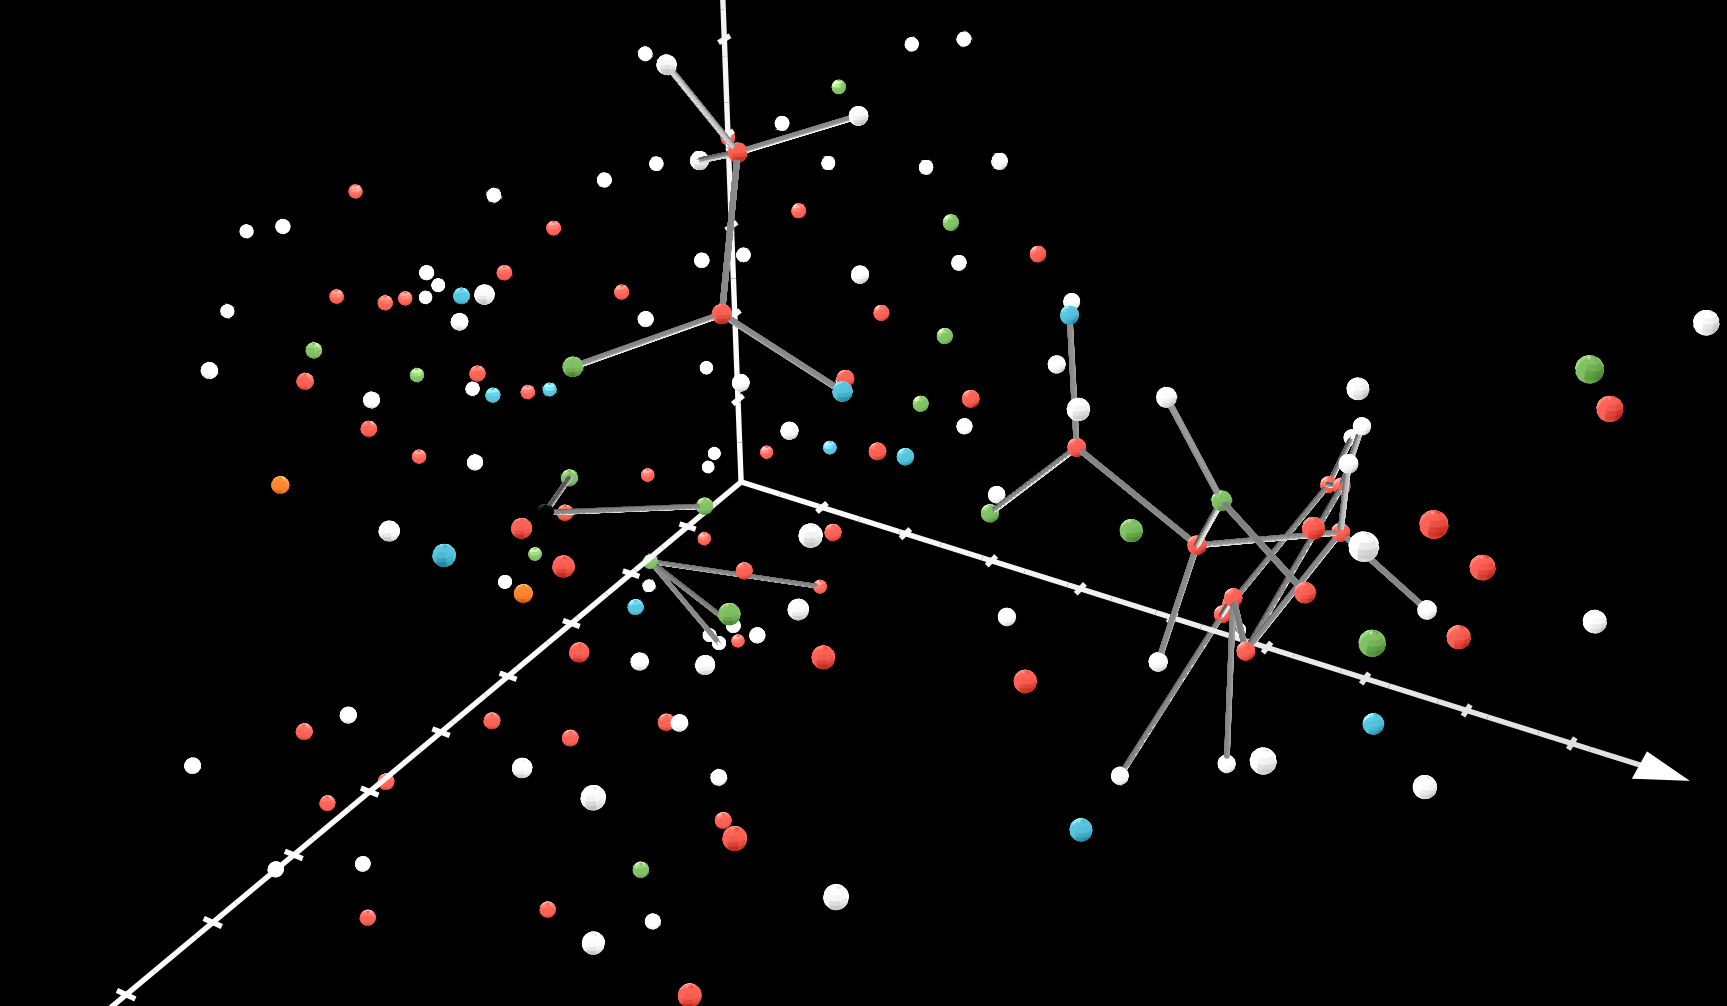
\includegraphics[width=4cm]{protein_peuliaisons_pres}
    \end{figure}
    \end{minipage}%
\end{frame}

\subsection{Notion de branche}
\begin{frame}{Branche sans ramification}
    \begin{minipage}{0.5\textwidth}%
        \begin{figure}[!htb]
            \centering
            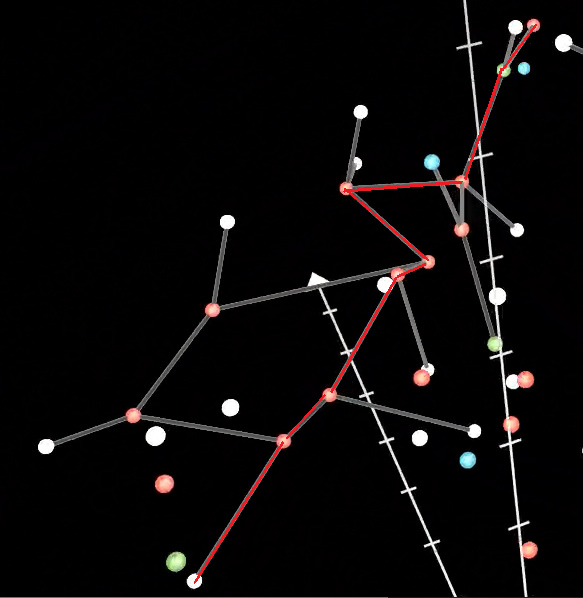
\includegraphics[width=5.5cm]{protein_branche}
        \end{figure}
    \end{minipage}%
    \hfill
    \begin{minipage}{0.4\textwidth}%
        On sélectionne une branche indépendamment du reste de la 
        protéine et du type des sommets
    \end{minipage}%
    \newline \newline \newline
    \underline{en python} : 
    \begin{itemize}
        \item type : \textcolor{airforceblue}{Coord} : $float\ *\ float\ *\ float$
        \item type : \textcolor{airforceblue}{Branche} : Coord list
            \newline \underline{ex} : $B = [(0,0,0), (1,1,1), (1.5,1,2)]$
    \end{itemize}
\end{frame}

\subsection{Coefficient}
\begin{frame}{Proximité de deux branches}
    \footnotesize
    \begin{minipage}{0.47\textwidth}%
    On considère 2 branches \textcolor{blue}{B1 en bleu} et \textcolor{violet}{B2 en violet} :
    \begin{itemize}
    \item même nombre d'atomes
    \item atomes ordonnés
    \item \underline{coloration distances}:
    du vert au rouge, moins élevé au plus élevé
    \end{itemize}
    \end{minipage}%
    \hfill
    \begin{minipage}{0.51\textwidth}%
        \begin{figure}[!htb]
            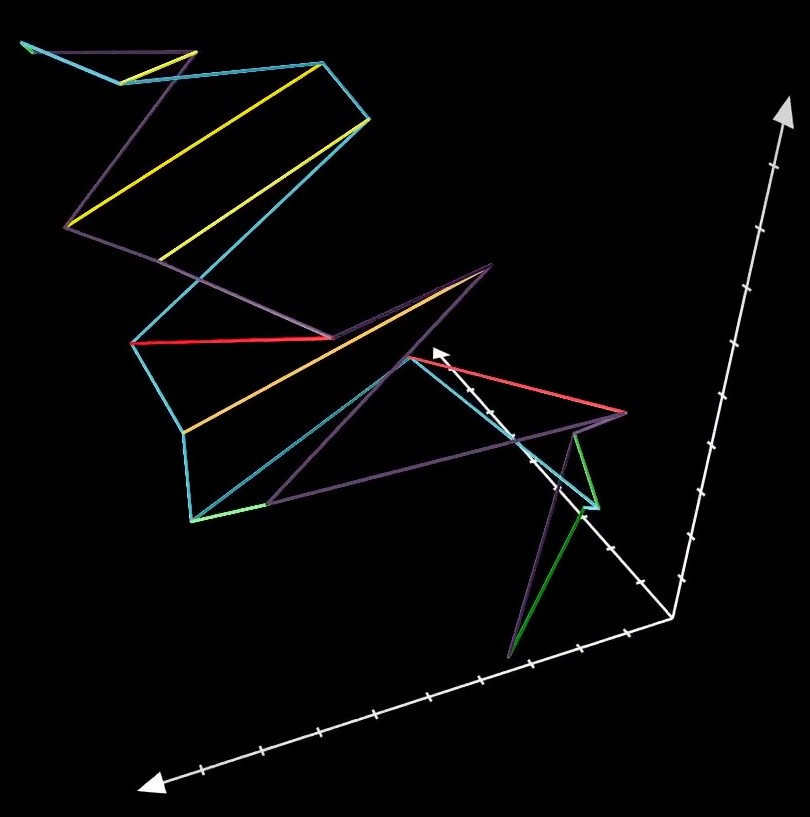
\includegraphics[width=5.3cm]{dlines_colored}
        \end{figure}
    \end{minipage}%
\end{frame}

\begin{frame}{Coefficient de proximité de branches}
    \footnotesize
    Soit $B_1 = [M_1,\cdots,M_n]$ et $B_2 = [N_1,\cdots,N_n]$ des branches
    \newline On pose, 
    \begin{align*}
    \forall i \in [\![1,n-1]\!],\ & l_i = M_iM_{i+1} \text{ et } l_i' = N_iN_{i+1}\\
    & d_i = max(l_i,l_i') \\
    & \theta_i = angle(  \overrightarrow{M_iM_{i+1}} ,   \overrightarrow{N_iN_{i+1}} ) 
    \end{align*}
    \begin{equation*}
        C_{dist} = \frac{\displaystyle\sum_{i=0}^{n-1} | \sin(\theta_{i}) | d_i}{\displaystyle\sum_{i=0}^{n-1} d_i} \qquad  
        C_{angle} = \frac{\displaystyle\sum_{i=0}^{n-1} |l_i' - l_i|}{\displaystyle\sum_{i=0}^{n-1} d_i}
    \end{equation*}
    \begin{equation*}
        R_{dist} = \frac{1}{1 + C_{dist}} \qquad R_{angle} = \frac{1}{1 + C_{angle}}
    \end{equation*}
    \newline Finalement, on définit : \newline
    \begin{equation*}
        \boxed{R = \frac{R_{dist}+R_{angle}}{2}}
    \end{equation*}
\end{frame}

\begin{frame}{Valeur du coefficient sur exemples}
    \begin{multicols}{2}
        \begin{figure}
            \centering
            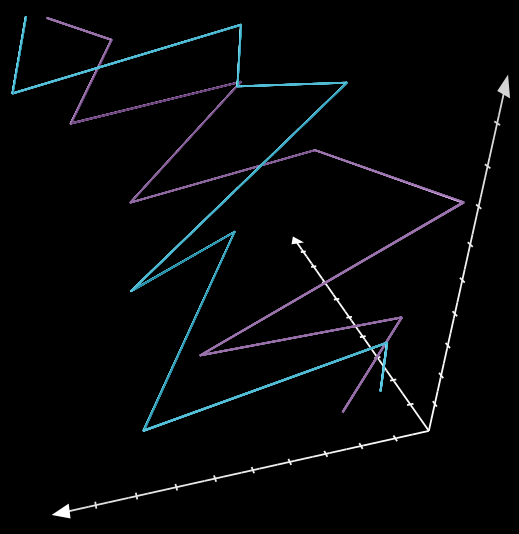
\includegraphics[width=3.5cm]{rcoeff_dist059_ang068_tot064}
        \end{figure}
    \vspace*{0.2cm}
        \begin{align*}
            R_{dist} = &0.59 \quad R_{angle} = 0.68 \\
            &\boxed{R = 0.64}
        \end{align*}
    \end{multicols}
    \begin{multicols}{2}
        \begin{figure}
            \centering
            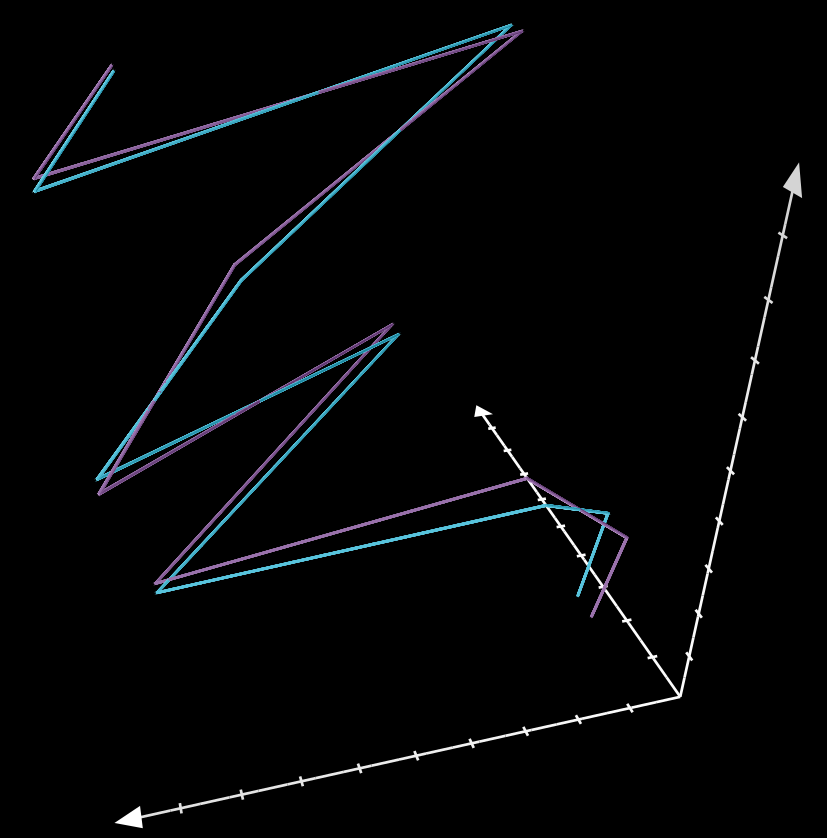
\includegraphics[width=3.5cm]{rcoeff_dist094_ang097_tot095}
        \end{figure}
    \vspace*{0.2cm}
            \begin{align*}
                R_{dist} = &0.94 \quad R_{angle} = 0.97 \\
                &\boxed{R = 0.95}
            \end{align*}
    \end{multicols}
\end{frame}

\begin{frame}{Des branches à la protéine complète}
    \normalsize
    \begin{figure}[!htb]
        \centering
        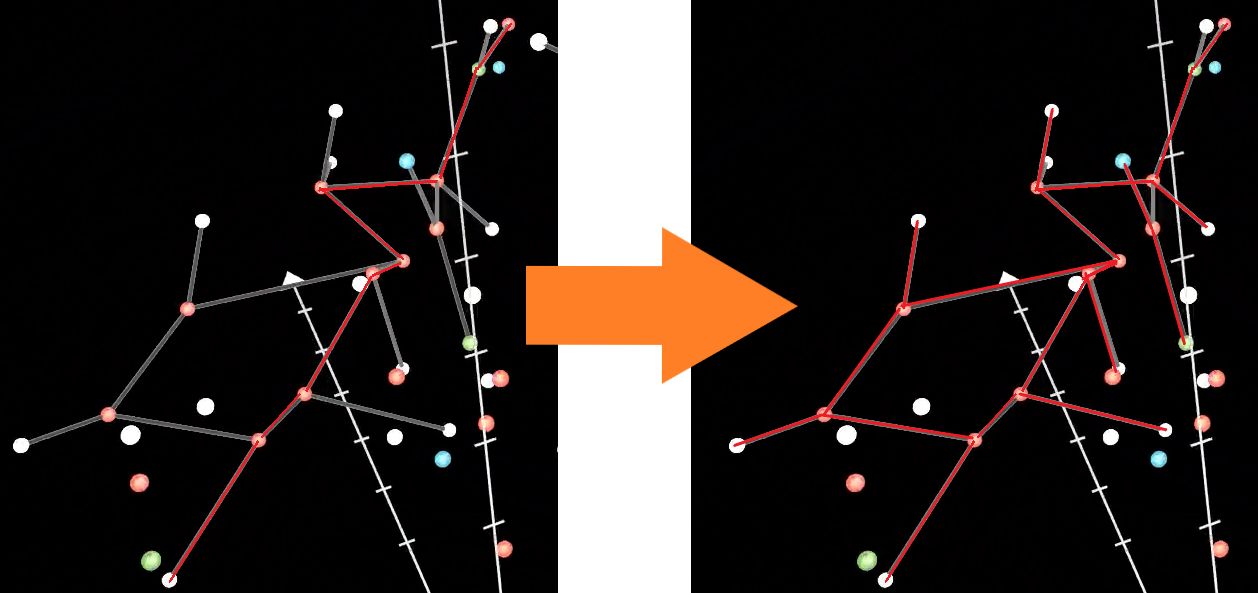
\includegraphics[width=10cm]{branche_to_prot}
    \end{figure}
\end{frame}

\section{Isomorphismes entre protéines}
\subsection{Définition}
\begin{frame}{Définition d'un isomorphisme de graphes}
\footnotesize
\fbox{%
\begin{minipage}{0.95\textwidth}

\underline{Définiton} : Soit $A_g$=$\lbrace g_1,\cdots,g_n \rbrace$ et $A_h$=$\lbrace h_1,\cdots,h_n \rbrace$ des ensembles
\newline Soit G=$A_g \times S_g$ et H=$A_h \times S_h$ 
deux graphes où $S_g,S_h\subseteq[n]\times[n]$ 
\newline ( ainsi, l'arête $(g_i,g_j)$ est dans G $\iff (i,j)\in S_g$ ) :
\begin{equation}
G \cong H\ si\ et\ seulement\ si\
\exists \sigma \in \Sigma _n, S_g = S_h^\sigma
\end{equation}
où $S_h^\sigma := \lbrace (\sigma(i),\ \sigma(j)),\ \exists (i,j) \in [\![1,n]\!]^2,\ (i,j) \in S_h \rbrace$
\end{minipage}
}
\newline
\newline
\underline{Exemple} :
    \begin{figure}[!htb]
        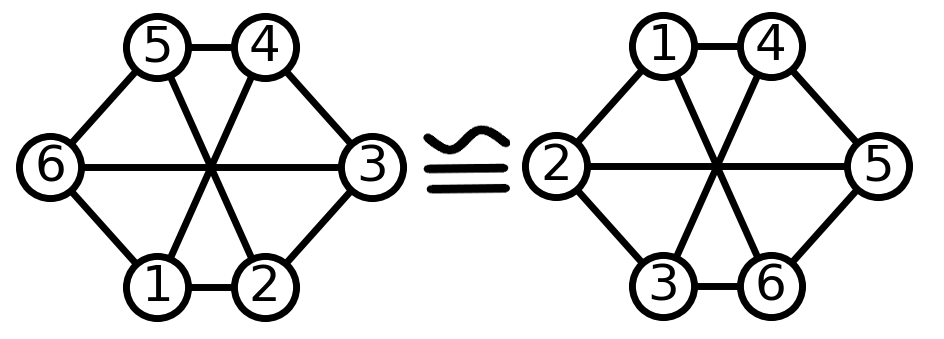
\includegraphics[width=9cm]{def_isom_ex1}
    \end{figure}
\end{frame}

\begin{frame}
    \begin{figure}[!htb]
        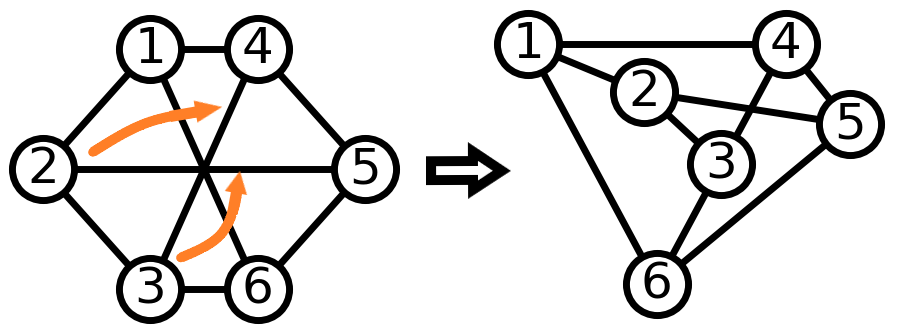
\includegraphics[width=9cm]{def_isom_ex2}
    \end{figure} 
    donc :
    \begin{figure}
        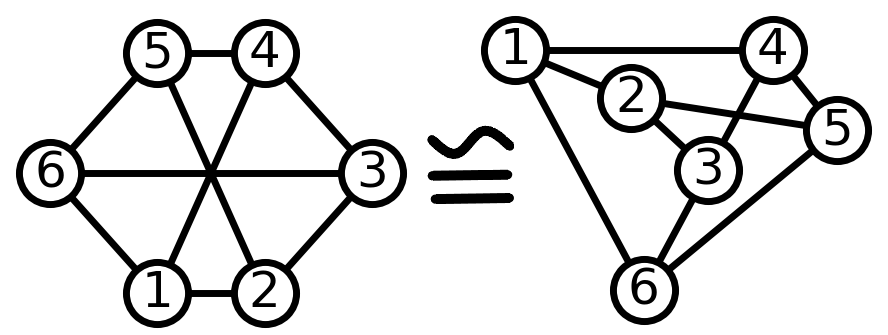
\includegraphics[width=9cm]{def_isom_ex3}
    \end{figure}
\end{frame}

\begin{frame}{Notion d'isomorphisme appliquée aux protéines}
    \small
    \begin{multicols}{3}
        \begin{figure}[!htb]
            \centering
            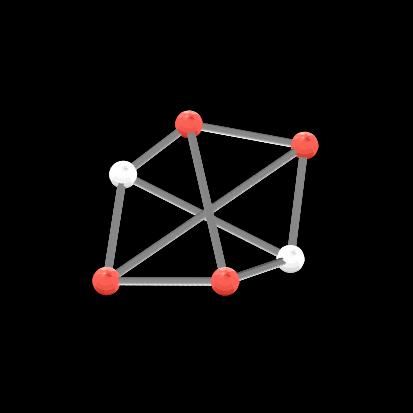
\includegraphics[width = 2.6cm]{prot_isom1}
        \end{figure}
        \begin{figure}[!htb]
            \centering
            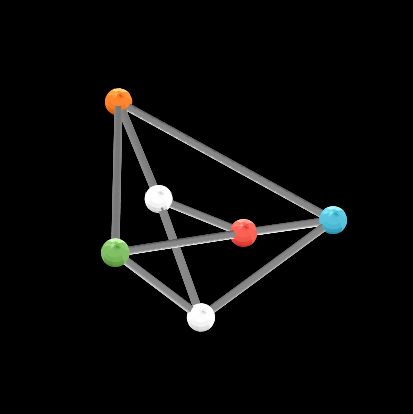
\includegraphics[width = 2.6cm]{prot_isom3}
        \end{figure}
        $\bullet$ Même structure 
        \newline $\bullet$ atomes différents
        \newline $\bullet$ positions des atomes différentes 
    \end{multicols}
    \begin{multicols}{3}
        \begin{figure}[!htb]
            \centering
            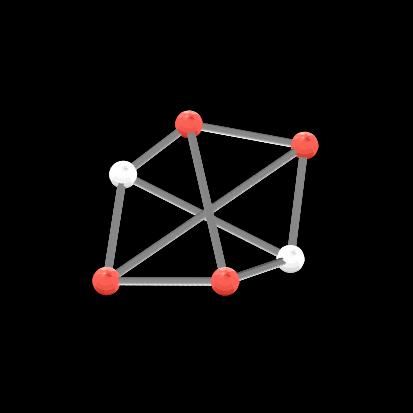
\includegraphics[width = 2.6cm]{prot_isom1}
        \end{figure}
        \begin{figure}[!htb]
            \centering
            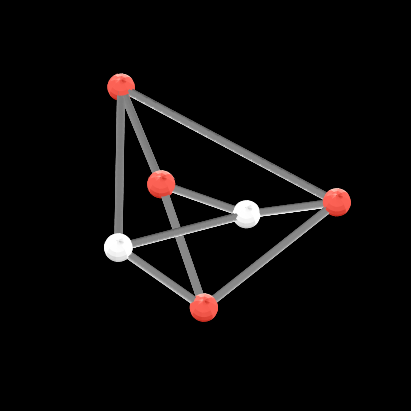
\includegraphics[width = 2.6cm]{prot_isom2}
        \end{figure}
        $\bullet$ Même structure 
        \newline $\bullet$ mêmes atomes
        \newline $\bullet$ positions des atomes différentes
    \end{multicols}
\end{frame}

\subsection{Force brute / tri des sommets}
\begin{frame}[fragile]{Idée 1 : Recherche par force brute}
\footnotesize
Pour simplifier, on considère G=$[\![ 1,n]\!]\times S_g$ et H=$[\![ 1,n]\!]\times S_h$ 
\newline\newline On cherche pour $\sigma \in \Sigma_n$, une permutation $\sigma$ telle que $S_g=S_h^\sigma$,

En python : 

\begin{itemize}
    \item type : \textcolor{charcoal}{Graph}
        \begin{tabular}{rl}
            \textcolor{airforceblue}{Graph.vertices} & $\longleftrightarrow \quad$ int list (liste des sommets) \\ 
            \textcolor{airforceblue}{Graph.edges} & $\longleftrightarrow \quad$ int list list (liste d'adjacence)
        \end{tabular}
        \newline\underline{ex} : $G_1 = Graph(\ [0,1,2],\ [[0,1], [0], [0]]\ )$
        \newline $\quad H_1 = Graph(\ [0,1,2],\ [[1,0], [2], [2]] )$
    \item type : permutation : int list
        \newline \underline{ex} : sur $\Sigma_3,\ Id = [0,1,2],\ \sigma_1=[2,1,0]$ la transpositon de 1 et 3
    \item fonction : \textcolor{airforceblue}{test$\_$isomorphism} : Graph, Graph, int list $\longrightarrow$ bool
        \newline \underline{ex} : $test\_isomorphism( G_1, H_1 , [0,1,2])$
        \newline teste si G et $H^{\sigma}$ sont les mêmes graphes
    \item fonction : \textcolor{airforceblue}{isomorphes} : Graph, Graph $\longrightarrow$ bool
        \newline \underline{ex} : $isomorphes(G, H) = True$
        \newline $G_1$ et $H_1$ sont isomorphes car $\exists \sigma \in \Sigma_3,\ (\sigma=\sigma_1)\ G_1=H_1^{\sigma}$
\end{itemize}
\end{frame}

\begin{frame}{Idée 2 : tri des sommets par invariants}
Les invariants des sommets que l'on peut utiliser sont par exemple le degré, le type du sommet,$\dots$ \newline\newline
\underline{Exemple} : G = $[\![1,5]\!] \times S_g$
\begin{align*}
\text{Les sommets ont une couleur : }
    & 1 ,\ 2\ \text{et}\ 4\ \text{sont bleus} \\
    & 3\ \text{et}\ 5\ \text{sont rouges}
\end{align*}
\begin{center}
Et ont aussi un degré égal au nombre de voisins
\end{center}
\begin{figure}[!htb]
    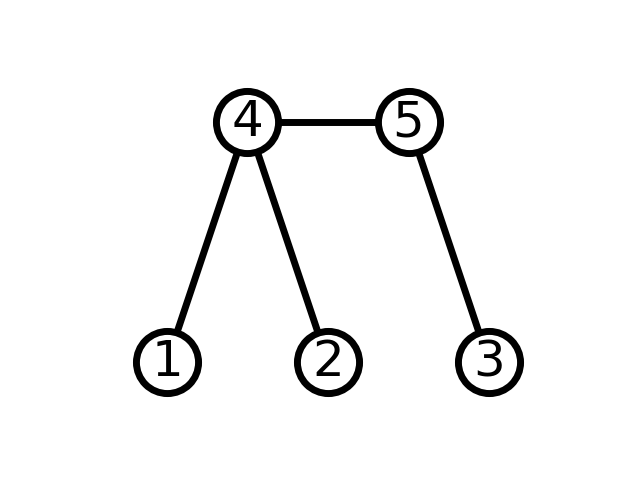
\includegraphics[width=5cm]{graph_tri.png}
\end{figure}


\end{frame}
\footnotesize
\begin{frame}
    \begin{center}
        On peut trier les sommets par couleurs : $(1\ 2\ 4\ |\ 3\ 5)$
        \begin{figure}[!htb]
        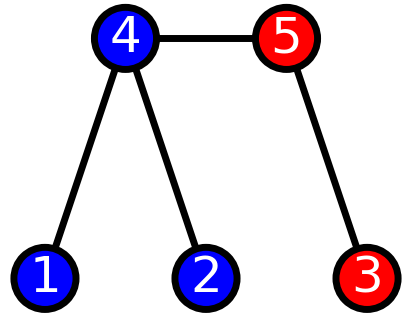
\includegraphics[width=2.5cm]{graph_tri_couleur.png}
        \end{figure}
        Ou trier les sommets par degré : $(1\ 2\ 3\ |\ 5\ |\ 4)$
        \begin{figure}[!htb]
        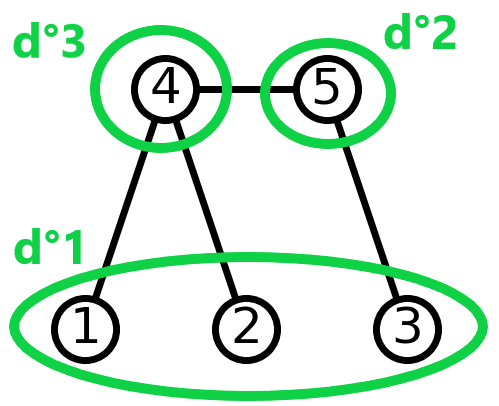
\includegraphics[width=2.8cm]{graph_tri_deg.png}
        \end{figure}
        Puis combiner les deux :  $(1\ 2\ |\ 3\ |\ 5\ |\ 4)$
        \begin{figure}[!htb]
        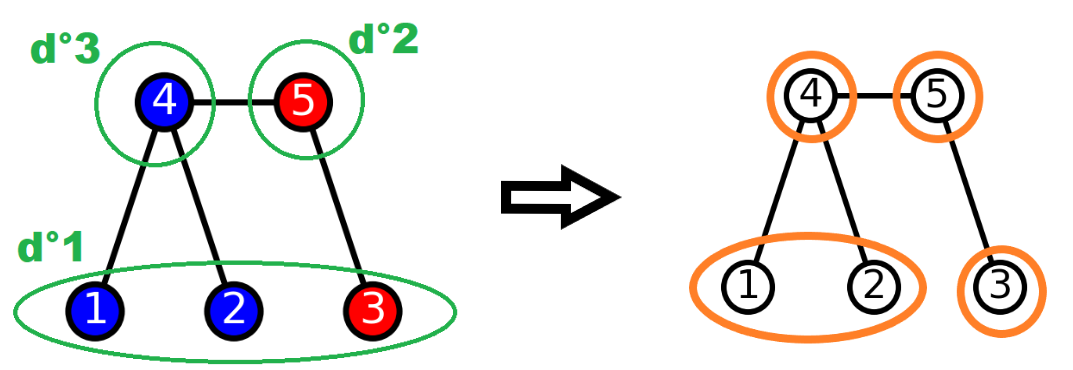
\includegraphics[width=7.1cm]{graph_tri_to_combin.png}
        \end{figure}
    \end{center}
\end{frame}

\begin{frame}{Idée 2 : tri des sommets par invariants}
Principe de recherche d'isomorphisme avec les sommets triés :
\begin{figure}[!htb]
    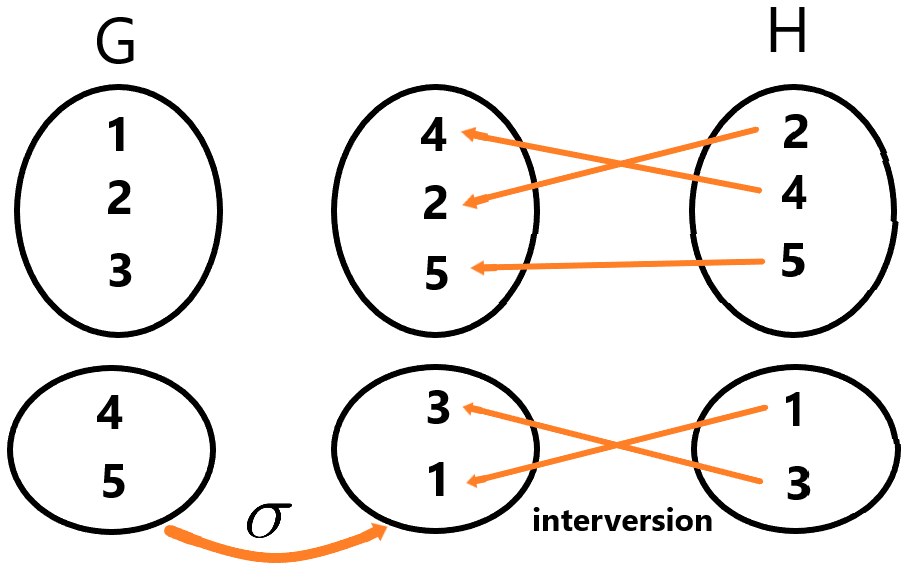
\includegraphics[width=9cm]{explication_tri.png}
    \end{figure}
\end{frame}

\begin{frame}{Idée 2 : tri des sommets par invariants}
    

\end{frame}

\begin{frame}{Tri sur les protéines}
    \begin{multicols\fbox{%
    \begin{minipage}{0.95\textwidth}
        On crée ainsi une partition de $[\![1,n]\!]$ des sommets $(V_1|\dots| V_t)$ pour G
        et $(W_1|\dots|W_t)$ pour H alors : \footnotesize
        \begin{equation}
            G \cong H \iff
            \exists (\sigma_i)_{i\in[\![ 1,t]\!]} \in 
            \Sigma _{|V_1|}\times..\times\Sigma _{|V_t|},\ 
            S_g=S_h^{\tilde{\sigma_1}\circ .. \circ \tilde{\sigma_t}}
        \end{equation} \footnotesize
        \begin{align*}
            avec\ \forall v_{i,j} \in V_i,\ \tilde{\sigma_i }(v_{i,j}) &= w_{i,\sigma_i(j)}\ 
            avec\ V_i=( v_{i,1}\ \dots\ v_{i,|V_i|} )\\
            \forall v \notin V_i,\ \tilde{\sigma_i }(v) &= v\
        \end{align*}
    \end{minipage}
    } \scriptsize \newline
\underline{Exemple} :
    \begin{align*}
        (V_1,V_2) &\to ( \quad 1 \quad 2 \quad 3 \quad| \quad 4 \quad 5\quad ) \\
        (W_1,W_2) &\to ( \quad 1 \quad 3 \quad 5 \quad| \quad 2 \quad 4\quad )
    \end{align*}
    \begin{center}
    \begin{tabular}{cccc}
        $\sigma_1$ 
        \footnote{
        $pour\ \sigma \in \Sigma_n ,\ on\ note\ \sigma = (\sigma(1)\ \sigma(2)\ \cdots\ \sigma(n)) $
        }
        & $\sigma_2$ & $(W_1^{\sigma_1}|W_2^{\sigma_2})$ & $\sigma = \tilde{\sigma_1} \circ \tilde{\sigma_2}$ \\
        \hline
        $(1\ 2\ 3)=Id$ & $(1\ 2)=Id$ & $( 1\quad 3\quad 5\ |\ 2\quad 4)$ & $(1\quad 3\quad 5\quad 2\quad 4)$ \\
        $(3\ 2\ 1)$ & $(1\ 2)=Id$ & $( 5\quad 3\quad 1\ |\ 2\quad 4)$ & $(5\quad 3\quad 1\quad 2\quad 4)$ \\
        $(1\ 2\ 3)=Id$ & $(2\ 1)$ & $( 1\quad 3\quad 5\ |\ 4\quad 2)$ & $(1\quad 3\quad 5\quad 4\quad 2)$ \\
    \end{tabular}
    \end{center}}{3}
    \begin{figure}[!htb]
        \centering
        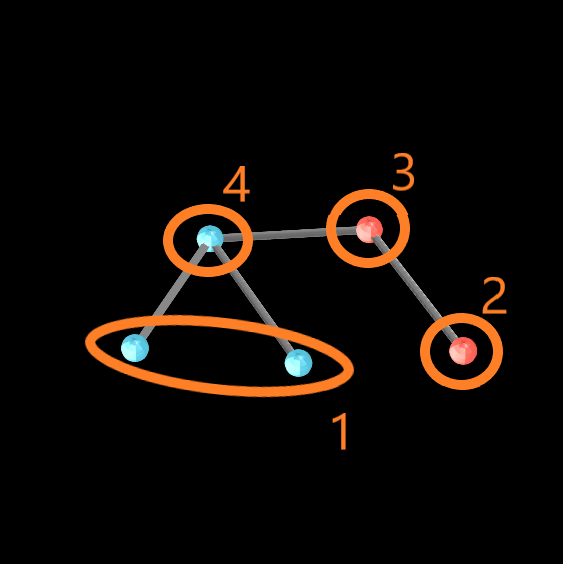
\includegraphics[width = 3cm]{prot_tri1}
    \end{figure}
    \begin{figure}[!htb]
        \centering
        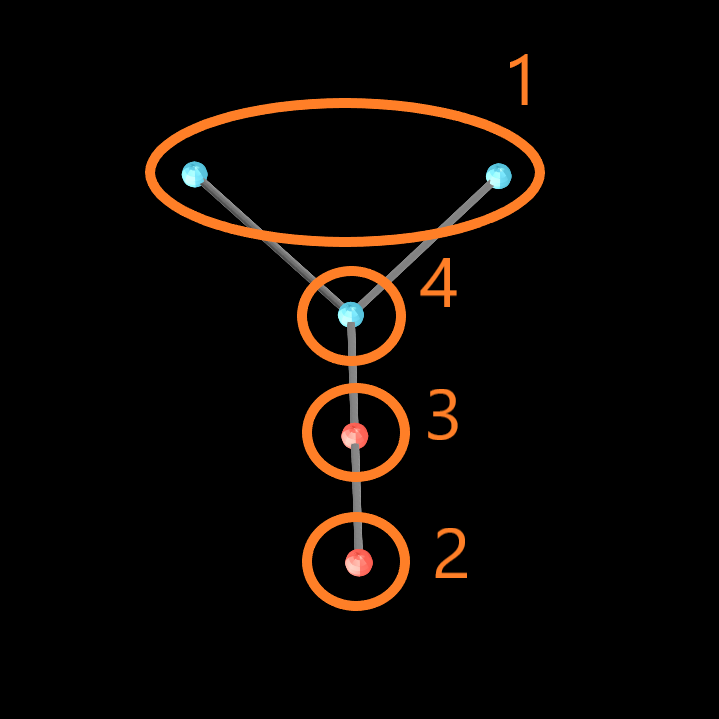
\includegraphics[width = 3cm]{prot_tri2}
    \end{figure}
    \begin{figure}[!htb]
        \centering
        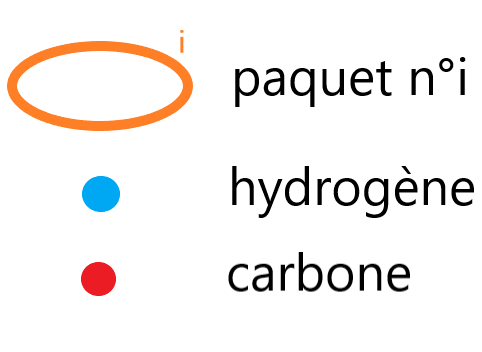
\includegraphics[width = 2cm]{legende_prot_tri}
    \end{figure}
    \end{multicols}
    \vspace*{1cm}
    \begin{minipage}{0.8\textwidth}
    \begin{center}
        \begin{tabular}{c|c|c}
            & force brute & tri \\
            \hline
            & & \\
            permutations & $5!=120$ & 2 \\
            de sommets & &
        \end{tabular}
    \end{center}
\end{minipage}
\end{frame}

\subsection{Comparaion}
\begin{frame}{Comparaison des complexités force brute / tri}
    G et H sont des graphes à n sommets tous deux \textbf{triés canoniquement}:
    \begin{itemize}
        \item types des $t \in \mathbb{N}$ paquets du tri sont dans le \textbf{même ordre} 
        \item on suppose les paquets de \textbf{même tailles} $t_i,\ i \in [\![1,t]\!]$ (sinon les graphes seraient trivialement non isomorphes)
        \newline 
    \end{itemize} 
    \scriptsize
    \begin{center}
    \begin{tabular}{c|c|c}
        & force brute & tri des sommets \\
        \hline & & \\
        procédé & permutations sur $\Sigma_n$ & combinaison de permutations sur \\
        d'itération & & $(\Sigma_i)_{i \in [\![1,t]\!]}$ tel que $\sum_{i=1}^t t_i  = n$ \\ & & \\
        \hline
        nombre & & \\ maximal & $n!$ & $\prod_{i=1}^t t_i!$ \\ d'itérations & & \\
        \hline
        mise en & & \\ mémoire & $\sum_{k=1}^n k! $ permutations & $\sum_{k=1}^{max(t_1,..,t_t)} k! $ permutations \\ nécéssaire
    \end{tabular}
    \end{center}
\end{frame}

\begin{frame}{Comparaison des complexités force brute / tri}
    On considère deux graphes triés en n paquets de taille q :
    \begin{figure}[!htb]
        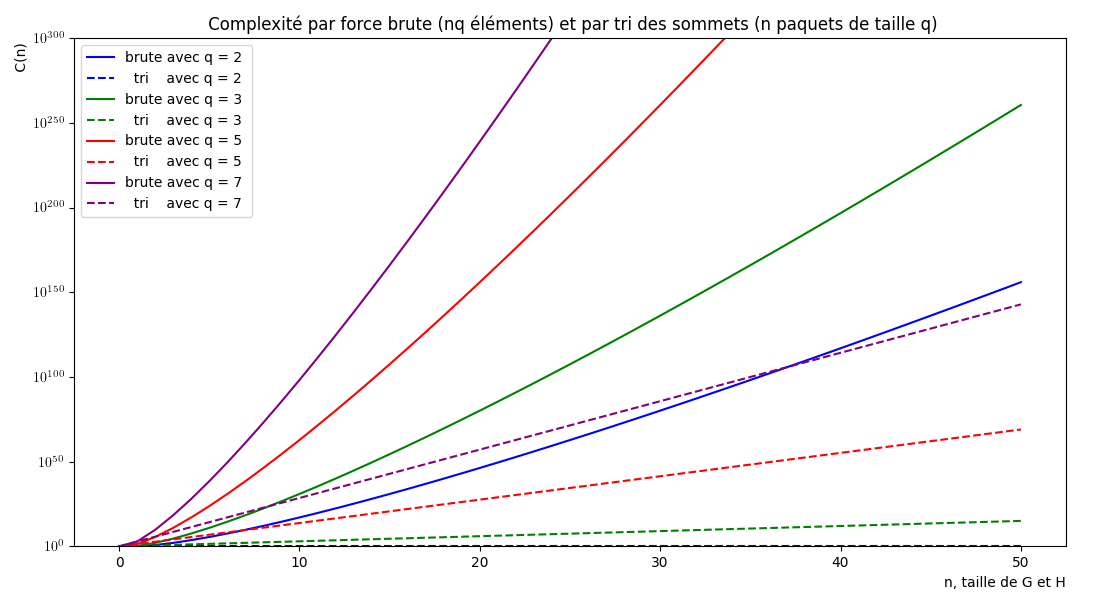
\includegraphics[width=10.3cm]{complexite_force_brute_tri_r.png}
    \end{figure}
\end{frame}

\section{Isomorphisme cannonique de McKay}

\begin{frame}{Idée 3 : Isomorphisme cannonique de McKay}
\begin{tabular}{ll}
\underline{Idée générale}: & $\bullet \quad$ tri équitable des sommets à partir d'un tri \\
& $\quad \rightarrow \quad$ informations avec la propagation du degré \\
& $\quad \rightarrow \quad$ tri optimal \\
& \\
& $\bullet \quad$ création d'un arbre de recherche de permutations \\
& $\quad \rightarrow \quad$ on crée artificiellement de nouveux tris équitables \\
& $\qquad \quad$ (fils de l'arbre) en isolant des sommets \\
& $\quad \rightarrow \quad$ les feuilles sont des tris ordonnés de parties à un \\ 
& $\qquad \quad$ sommet : ce sont des permutations \\
& $\bullet \quad$ définition d'un ordre total sur les graphes \\
& $\quad \rightarrow \quad$ déterminer le plus grand pour cette relation parmi \\
& $\qquad \quad$ les graphes permutés avec les feuilles de l'arbre \\
& $\quad \rightarrow \quad$ on obtient alors l'\underline{isomorphisme cannonique}
\end{tabular}
\end{frame}

\subsection{Tri équitable}
\begin{frame}{Tri des sommets encore plus fin}
    \begin{center}
        \underline{Utilisation de la propagation du degré} :
    \end{center}
    Tri des sommets des paquets par degré dans les autres paquets pour en faire un nouveau tri \newline
    $\quad \rightarrow \ $ jusqu'à ce qu'il n'y ait plus de simplifications possibles \newline \newline
    \underline{Exemple} :
    \begin{align*}
        \text{Soit } \pi &= (1\ |\ 3\ 7\ 9\ |\ 6\ 8\ |\ 2\ 4\ |\ 5) \text{ un tri des sommets du graphe G} \\
        &= (V_1\ |\ V_2\ |\ V_3 \ | \ V_4\ |\ V_5)
    \end{align*} 
    \begin{minipage}{0.3\textwidth}
        \begin{figure}
        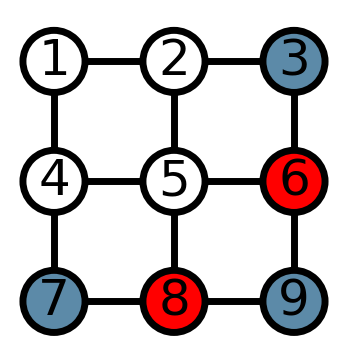
\includegraphics[width = 3cm]{graph_tri_equal_colored} 
        \caption{\label{fig:graphe_tri_equal}Graphe G}
        \end{figure}
    \end{minipage}
    \begin{minipage}{0.25\textwidth}
        \begin{align*}
            \textcolor{airforceblue}{V_2} & \textcolor{airforceblue}{=(3 \ 7\ 9)} \\
            \textcolor{red}{V_3}  & \textcolor{red}{=(6\ 8)}
        \end{align*}
    \end{minipage} 
    \begin{minipage}{0.4\textwidth}
        \begin{align*}
        & \text{Tri de } V_2 \text{ par degré dans } V_3 : \\ \\
        & deg(3,V_3)=deg(7,V_3)=1 \\
        & deg(9,V_3)=2 \\
        & \text{donc } V_2 = (3\ 7\ |\ 9)
        \end{align*}
        \begin{center}
            $\pi ' = (1\ |\ 3\ 7\ |\ 9\ |\ 6\ 8\ |\ 2\ 4\ |\ 5)$
        \end{center}
    \end{minipage}
    \begin{center}
    tri $\pi'$ plus fin
    \end{center}
\end{frame}

\begin{frame}{Tri des sommets encore plus fin : tri équitable}
    \underline{Tri équitable} : la propagation de degré ne donne plus de nouveau tri
    \begin{align*}
        & \forall (i,j)\in[\![1,n]\!]^2, \text{ tous les sommets de } V_i \text{ ont le même degré dans } V_j \\
        \iff \ & \forall (i,j)\in[\![1,n]\!]^2,\ 
        \forall (v,w) \in V_i^2,\ deg(v,V_j)=deg(w,V_j) \\
    \end{align*}
    Soit $\pi$ un tri, on note :
    \begin{equation}
        \boxed{R(\pi) \text{ le plus grand} \footnote{défini selon un ordre partiel sur les partitions}
        \text{ tri équitable ordonné obtenu à partir de \pi}}
    \end{equation} 

\end{frame}

\subsection{Arbre de recherche}
\begin{frame}{Arbre de recherche de permutations}
    \begin{minipage}{0.3\textwidth}
        \begin{figure}[!htb]
            \centering
            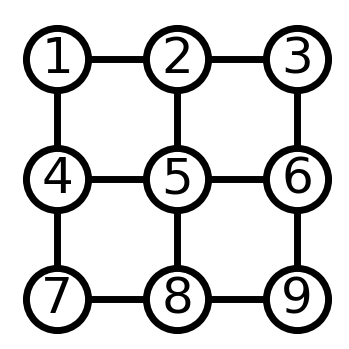
\includegraphics[width = 1.7cm]{graph_tri_equal}
            \caption{\label{fig: Graph G2}Graph G}
        \end{figure}
    \end{minipage}
    \begin{minipage}{0.6\textwidth}
        \begin{center}
            On considère le tri suivant le degré :\newline
            $\pi = (1\ 3\ 7\ 9\ |\ 2\ 4\ 6\ 8\ |\ 5)\qquad $ \newline \newline
            $R(\pi)=\pi$ est alors la racine de l'arbre
        \end{center}
    \end{minipage}
    \newline \newline \newline
    \underline{Trouver les fils} :
    \begin{itemize}
        \item trouver la première partie $V_i$ d'au moins 2 éléments de $\pi$
        \item pour $v \in V$, on crée \textbf{artificiellement} un nouveau tri équitable :
        $\quad \longrightarrow \quad \pi_v = \pi \perp v = R(\ (V_1|..|\ \lbrace v \rbrace \ |\ V_i \textbackslash \lbrace v \rbrace\ |..)\ )$
        \item chacun des tris créés est un fils, on réitère jusqu'à obtenir des tris triviaux (paquets de taille 1)
    \end{itemize}
\end{frame}

\begin{frame}{Arbre de recherche de permutations}
    \begin{figure}[!htb]
        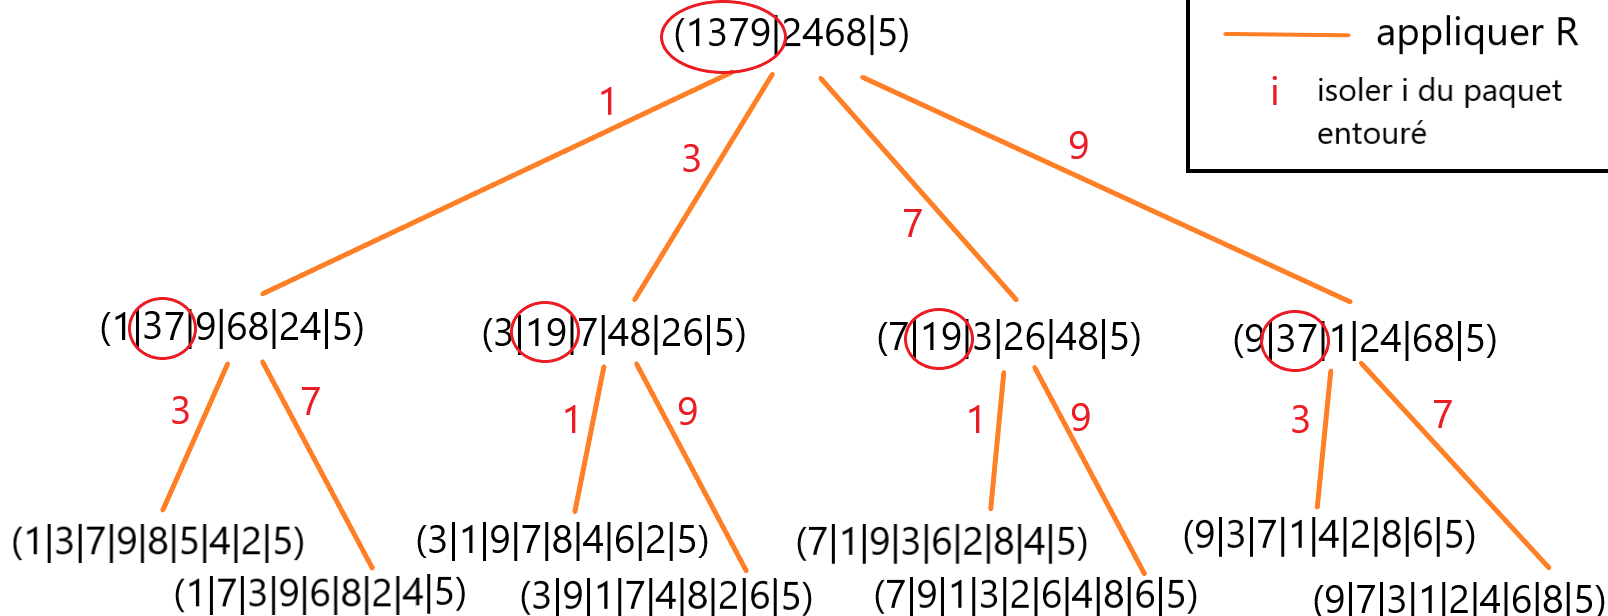
\includegraphics[width = 10cm]{search_tree}
        \caption{\label{fig:Arbre T(G)} Arbre T(G) de racine $\pi=(1\ 3\ 7\ 9\ |\ 2\ 4\ 6\ 8\ |\ 5)$}
    \end{figure}
\end{frame}

\subsection{Isomorphisme cannonique}
\begin{frame}{Relation d'ordre sur les graphes et isomorphisme cannonique}
    \underline{Ordre total $\preceq$ sur les graphes} : \newline \newline
    On pose la fonction $i:\ G\ \longmapsto i(G)$ telle que : \newline
    $\quad \bullet \ i(G)$ est la séquence binaire $(\mathds{1}_{(i,j)\in G})$ dans l'ordre lexicographique \newline
    $\quad \bullet \ G \preceq H$ si et seulement si $i(G) \leq i(H)$ en décimal
    \newline \newline
    On pose alors l'\textbf{ismorphisme cannonique de McKay} (pour le tri $\pi$):
    \begin{equation}
        \boxed{C_M(G) = max_{\preceq}\ \lbrace G^{\sigma},\ \sigma \text{ noeud terminal de T(G) de racine } \pi \rbrace }
    \end{equation}
    alors:
    \begin{equation}
        \boxed{G \cong H \text{ si et seulement si } C_M(G) = C_M(H)}
    \end{equation}
    \newline
    \underline{Exemple} : pour $\pi = (1\ |\ 3\ 7\ |\ 9\ |\ 6\ 8\ |\ 2\ 4\ |\ 5)$
    \begin{multicols}{2}
        \begin{figure}[!htb]
            \centering
            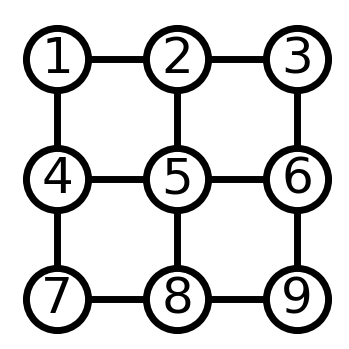
\includegraphics[width = 2.5cm]{graph_tri_equal}
            \caption{\label{fig: Graphe G}Graphe G}
        \end{figure}
        \vspace*{1cm}
        \begin{figure}[!htb]
            \centering
            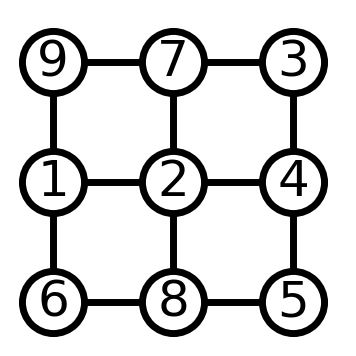
\includegraphics[width = 2.5cm]{cmg}
            \caption{\label{fig: Isomorphe G} Graphe $C_M(G)$}
        \end{figure}
    \end{multicols}
\end{frame}

\subsection{Application}
\begin{frame}{Application sur les protéines}
    \begin{multicols}{2}
        \begin{figure}[!htb]
            \centering
            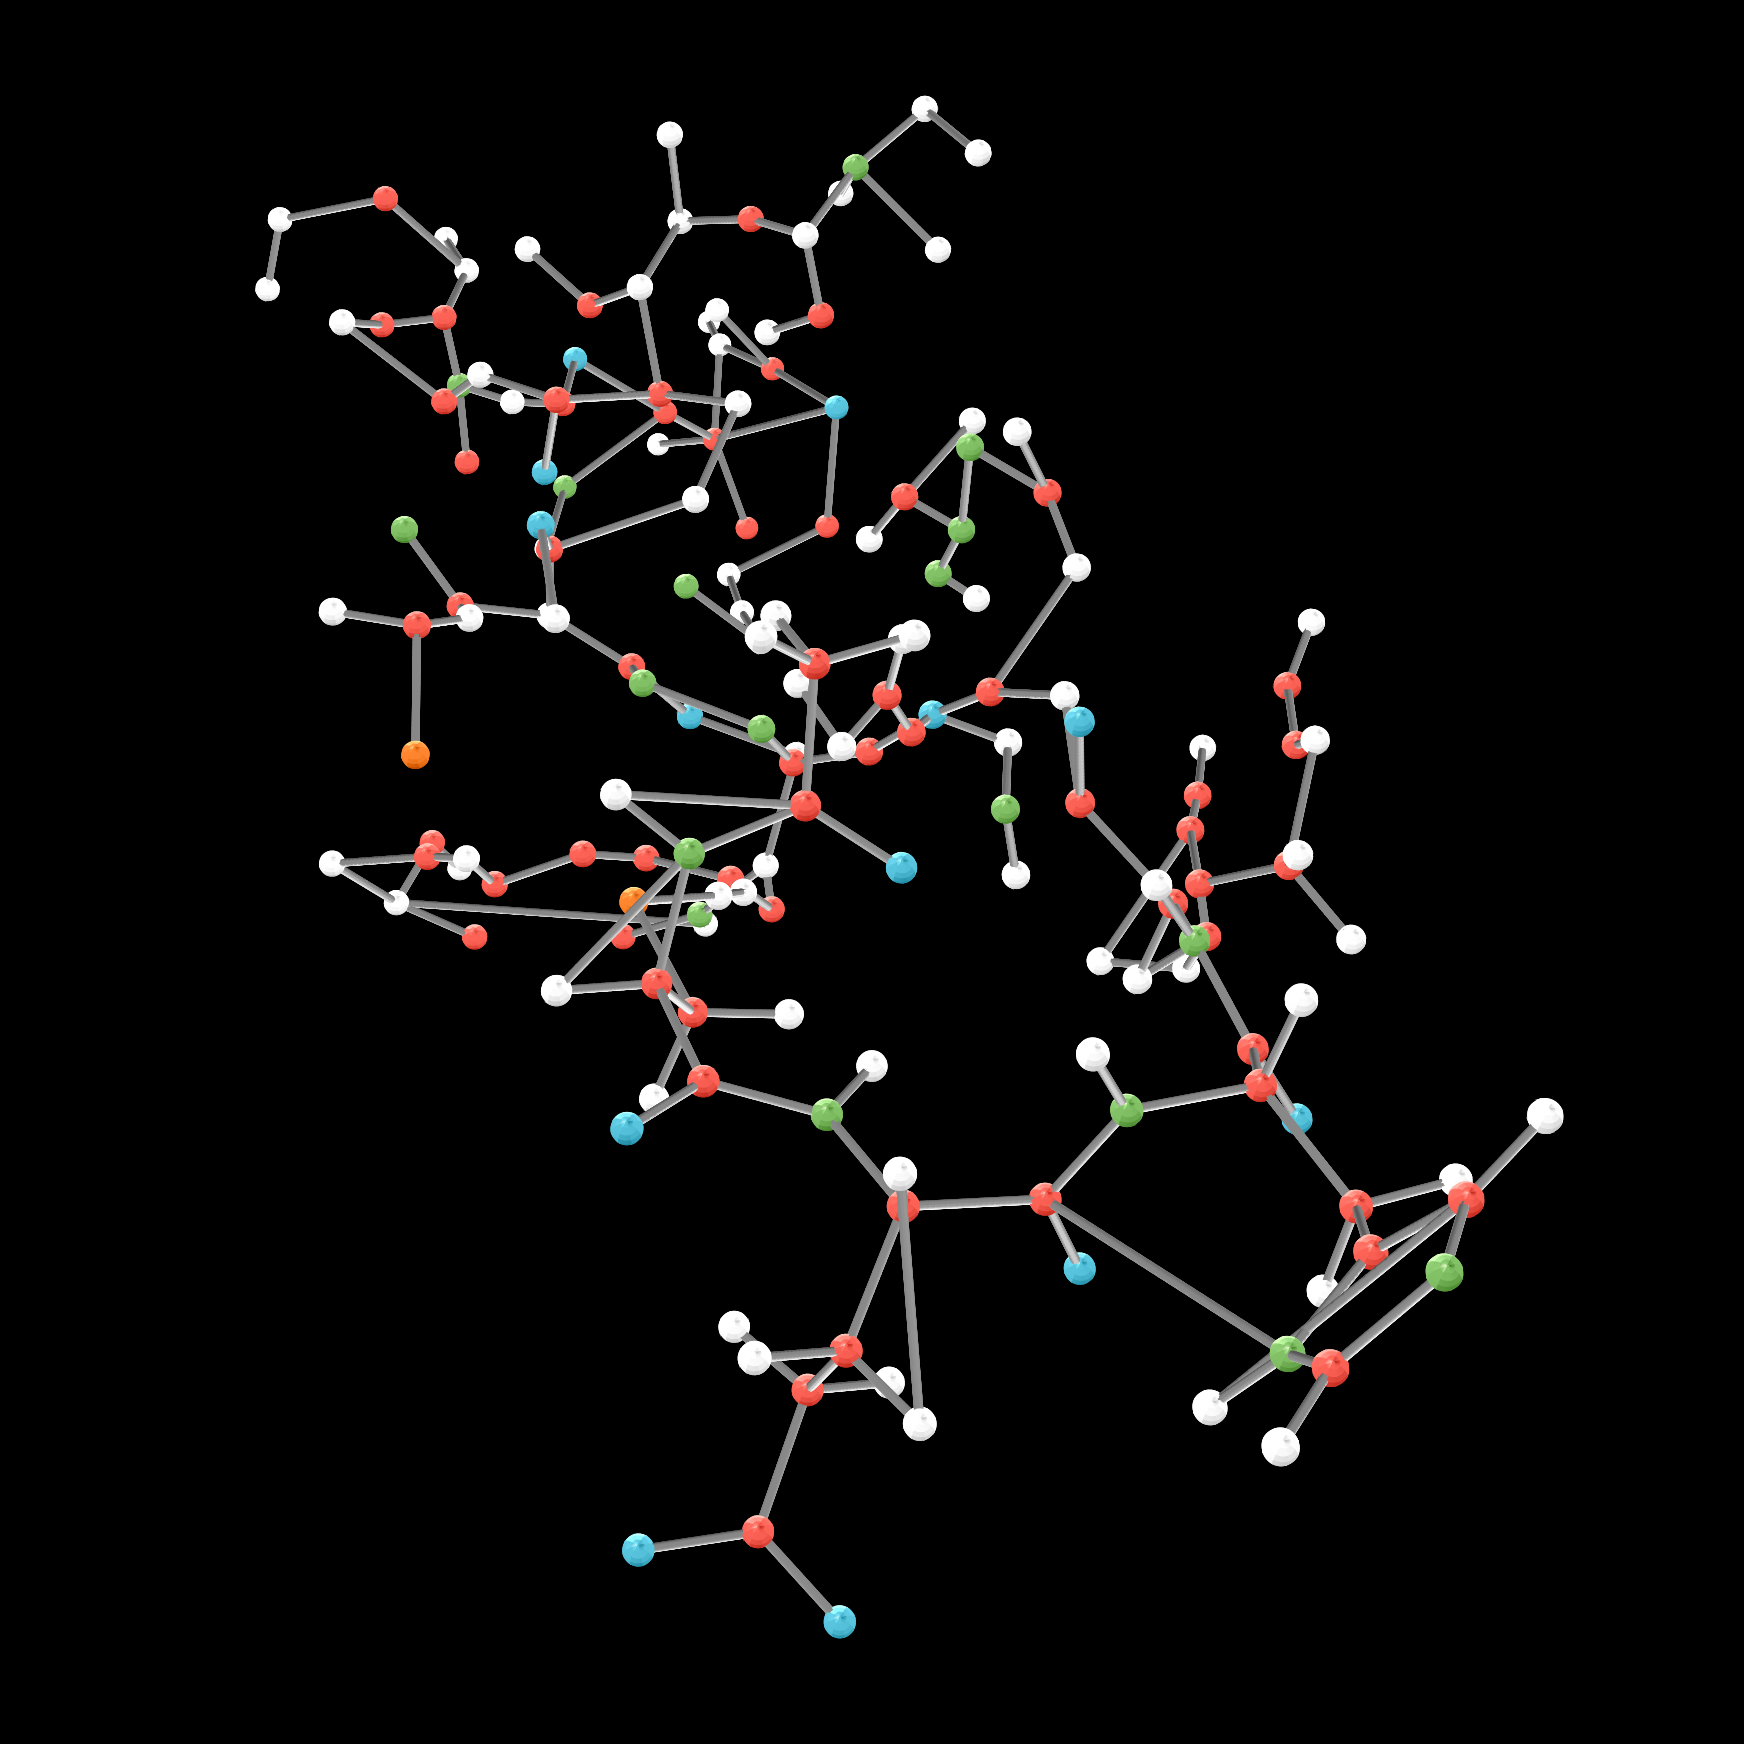
\includegraphics[width = 3cm]{protein_cov}
            \caption{\label{fig: Protéine}Protéine}
        \end{figure}
        \begin{center}
        \begin{figure}[!htb]
            \centering
            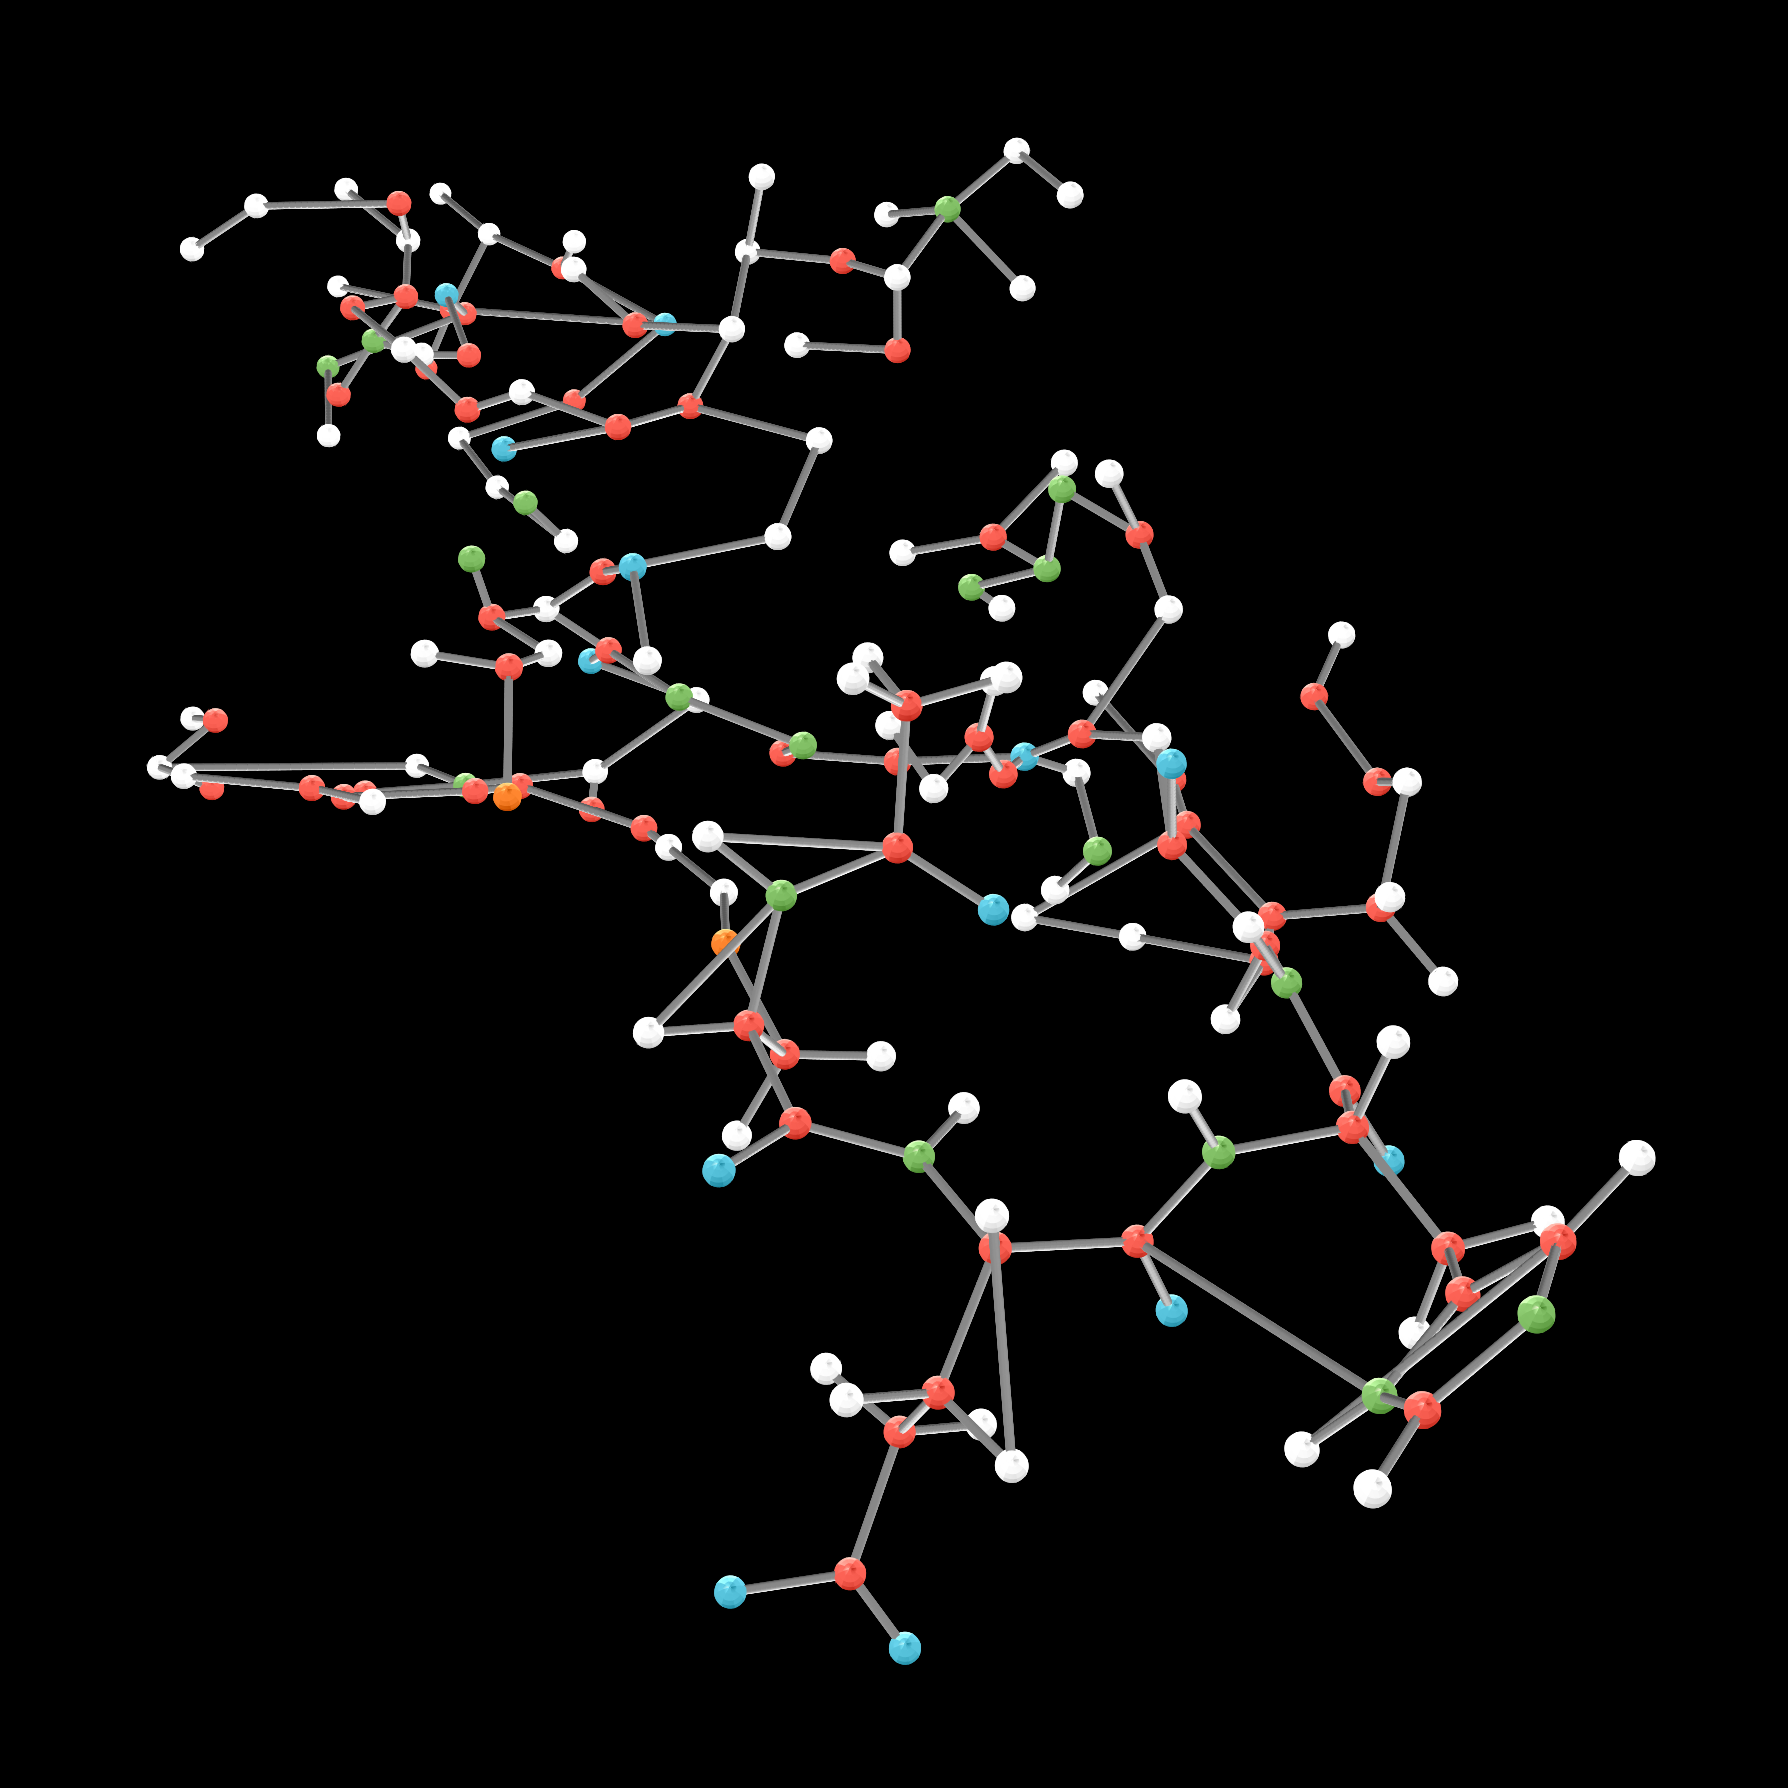
\includegraphics[width = 3cm]{protein_cov_translatee}
            \caption{\label{fig: Protéine translatée}Même protéine mais déplacée et numérotation différente des sommets}
        \end{figure}
    \end{center}
    \end{multicols}
    \underline{Temps d'éxecution} : pour cette protéine de 171 atomes
    \begin{center}
    \begin{tabular}{c|c}
        tri par degré et atomes & 0.002 s\\
        propagation des degrés & 7.4 s \\
        test d'isomorphisme & 0.3 s \\
        temps total d'éxecution & 7.8 s
    \end{tabular}
    \end{center}
    \underline{Résultat} : protéines isomorphes et permutation renvoyée correcte
    \newline tri + propagation du degré $\rightarrow$ paquets d'au plus 4 atomes
\end{frame}

\section{Comparaion de protéines}

\subsection{Structure}
\begin{frame}{Recherche du plus grand sous-graphe isomorphe}
    \scriptsize
    \begin{figure}[!htb]
    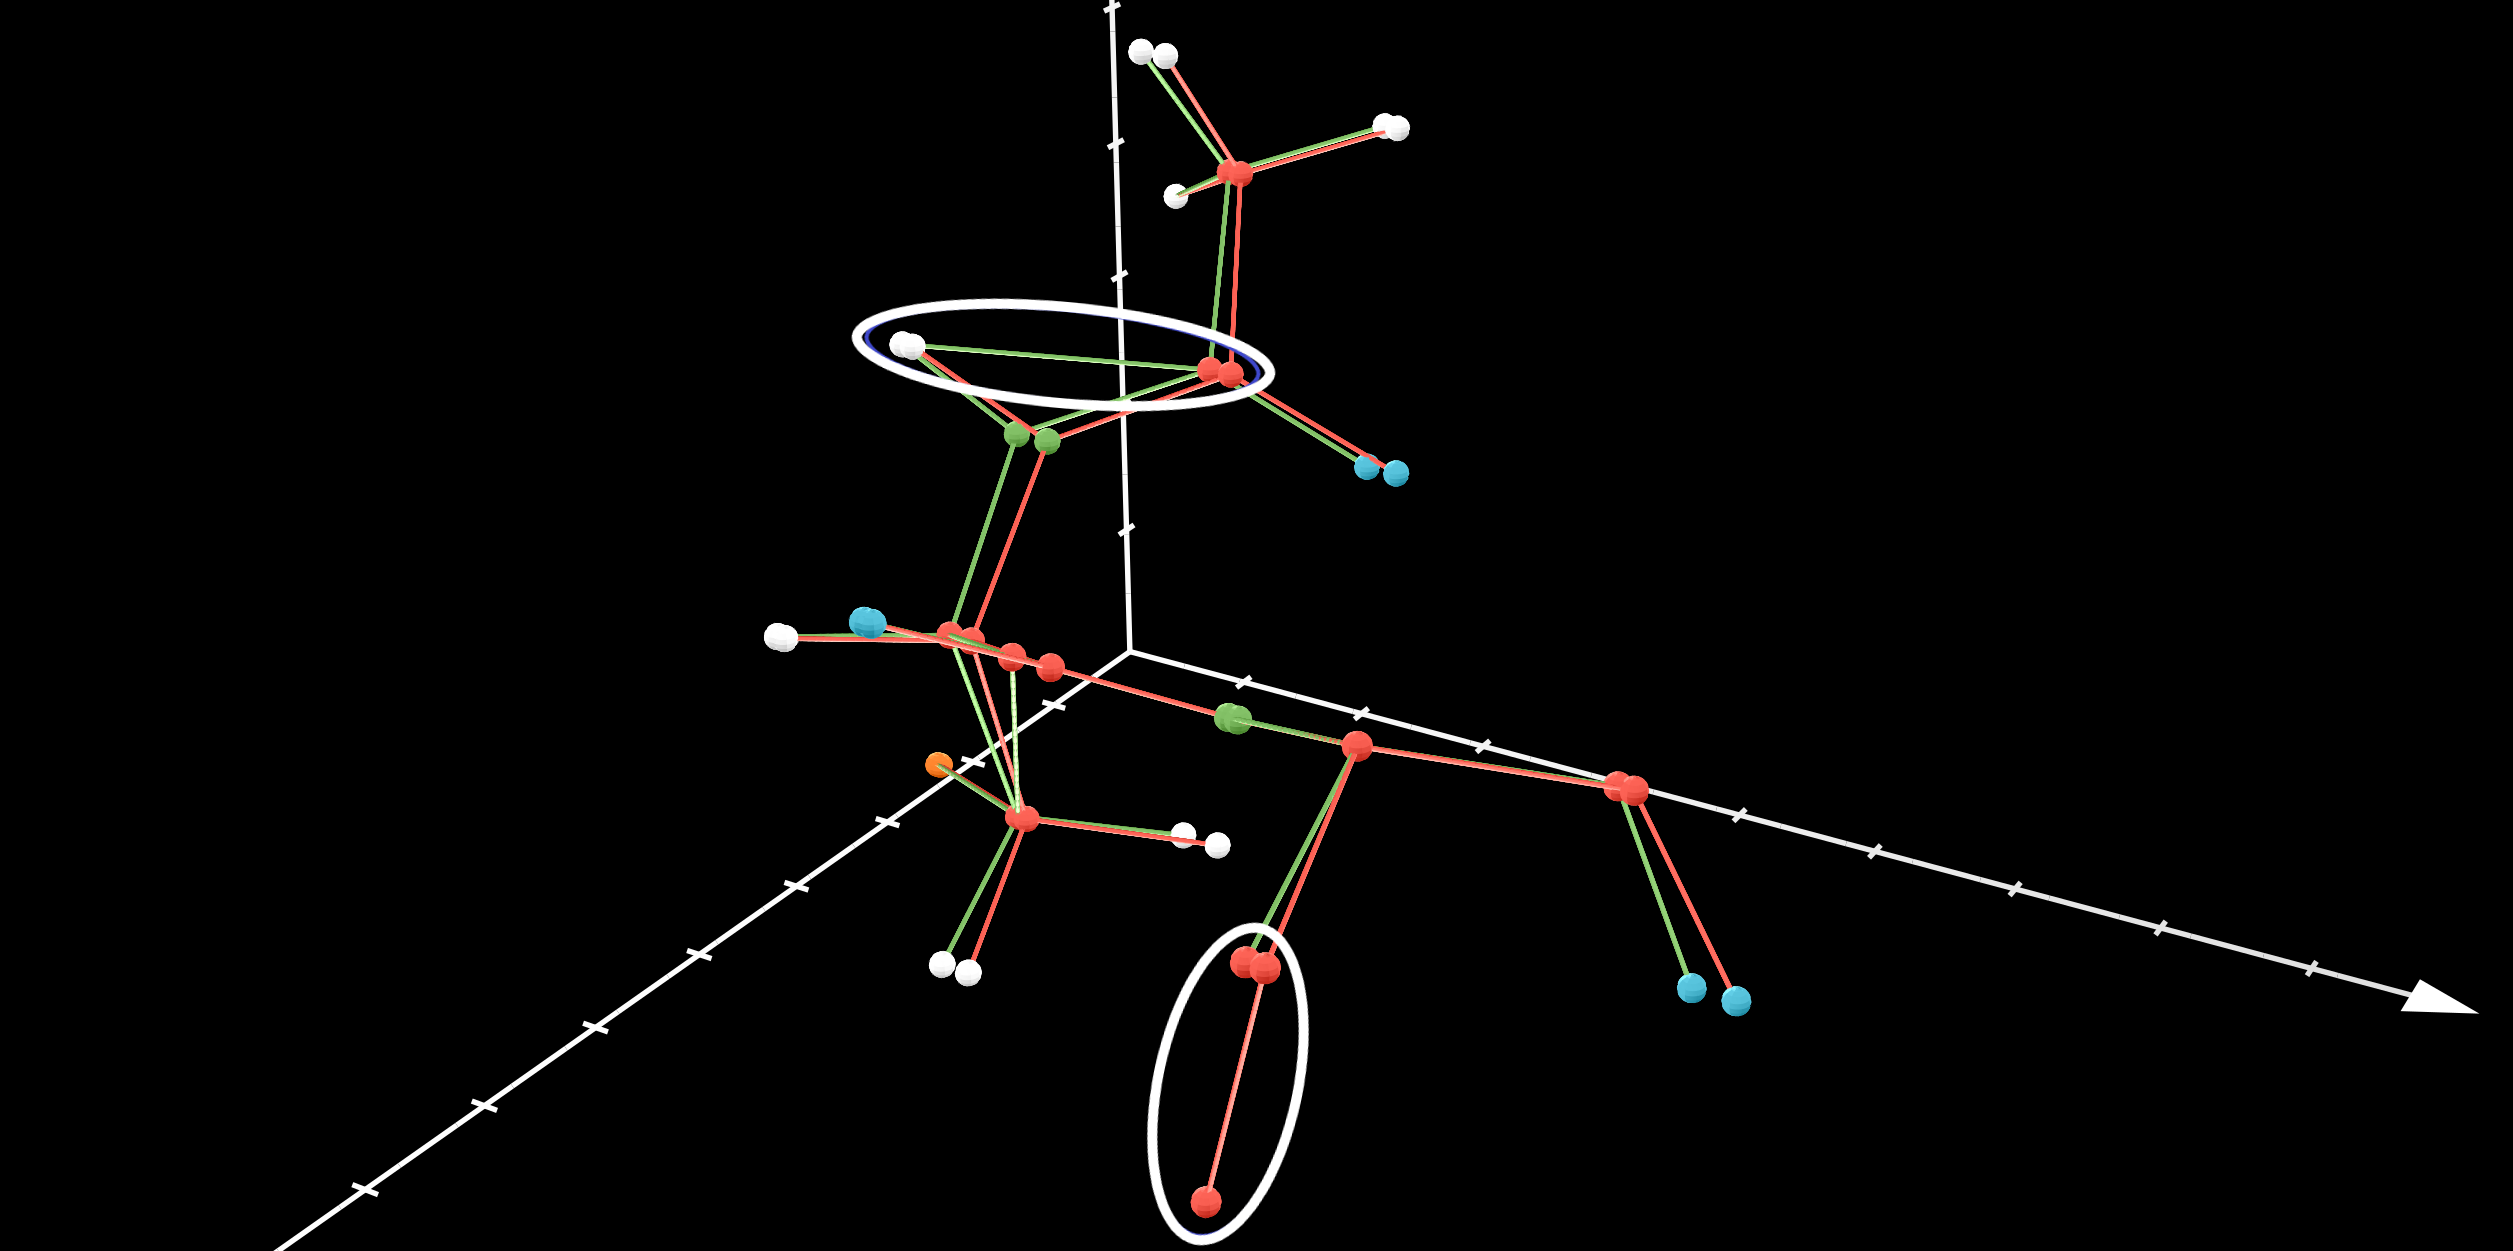
\includegraphics[width = 8.6cm]{comp_sub_largeview}
    \end{figure}
    \begin{multicols}{2}
        \begin{figure}[!htb]
            \centering
            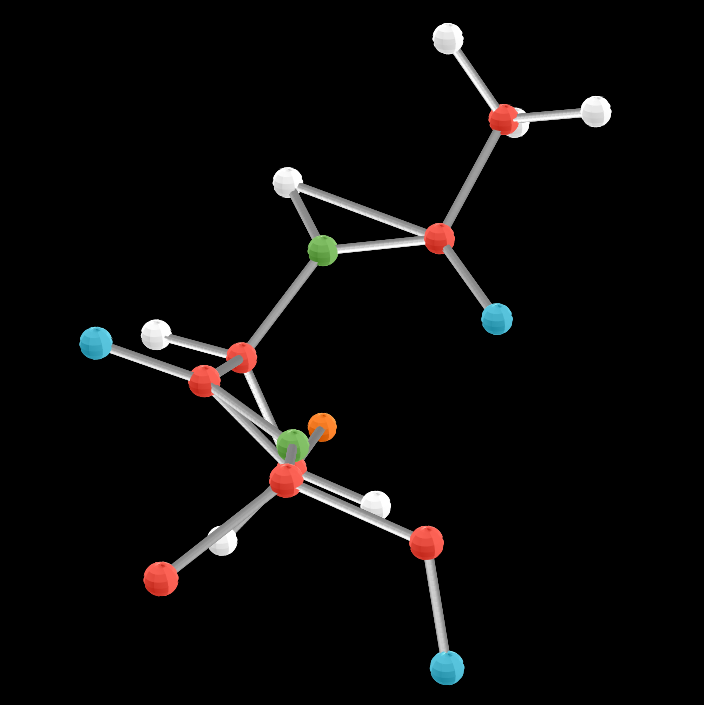
\includegraphics[width = 3cm]{sub1_lim22}
            \caption{\label{fig: sub1}Protéine de 21 atomes (en vert)}
        \end{figure}
        \begin{figure}[!htb]
            \centering
            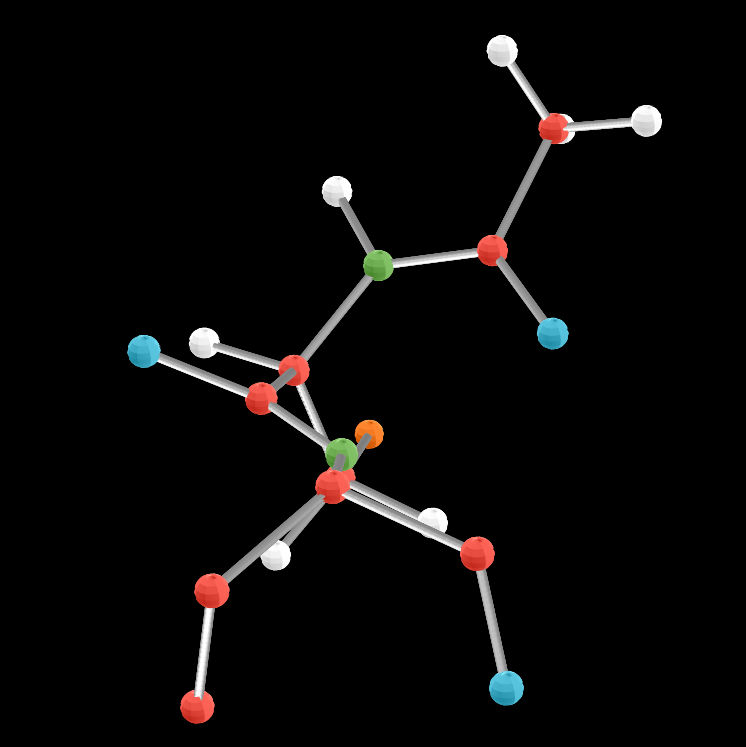
\includegraphics[width = 3cm]{sub2_lim22}
            \caption{\label{fig: sub2}Protéine de 22 atomes (en rouge)}
        \end{figure}
    \end{multicols}
\end{frame}

\begin{frame}{Recherche du plus grand sous-isomorphe}
    \begin{multicols}{2}
        \begin{figure}[!htb]
            \centering
            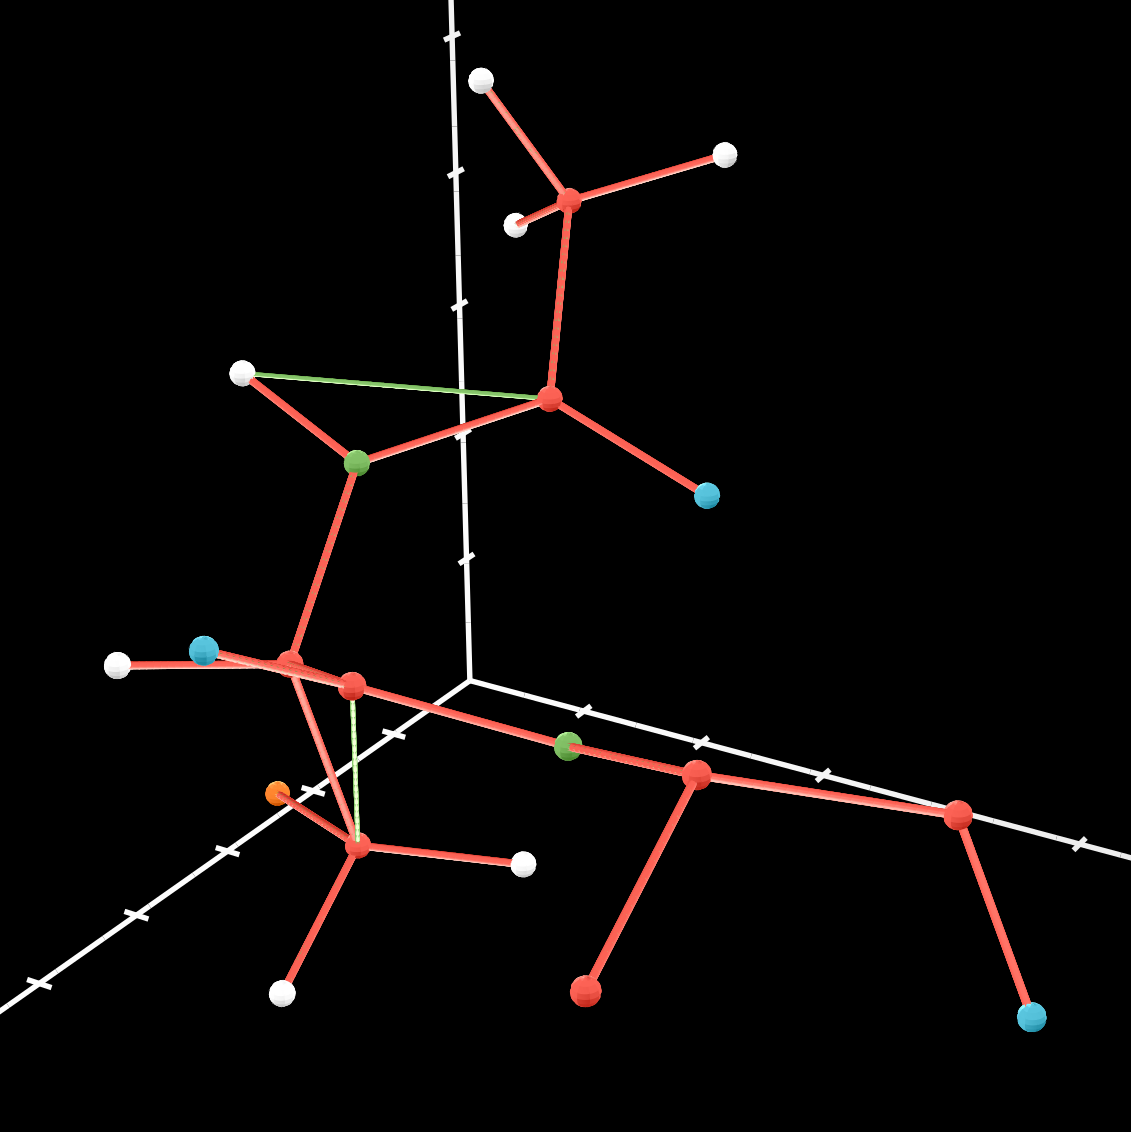
\includegraphics[height=4cm]{subgraph_lim22_1}
        \end{figure}
        \begin{figure}[!htb]
            \centering
            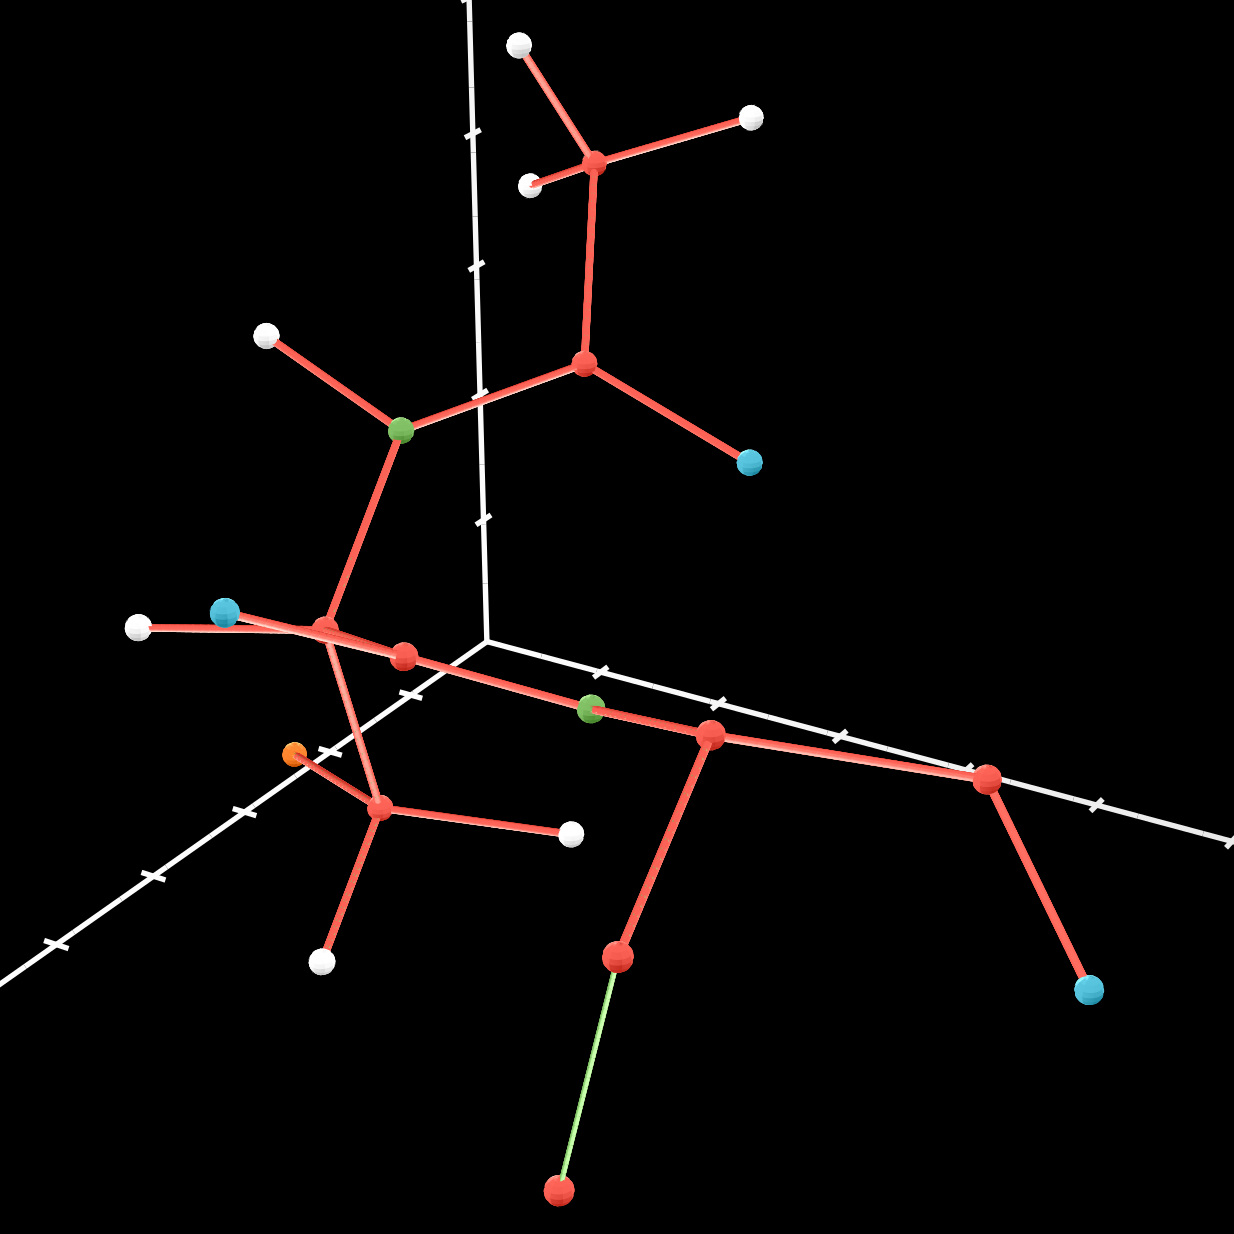
\includegraphics[height=4cm]{subgraph_lim22_2}
        \end{figure}
    \end{multicols}
    \begin{figure}
        \centering
        \caption{\label{fig:max_isom}Un sous-graphe isomorphe de taille maximale}
    \end{figure} 
    temps d'éxecution sur ce modèle : 3-4 minutes
    \begin{center}
        Cas d'égalité, sous-graphes de même taille ?
    \end{center}
\end{frame}

\subsection{Position}
\begin{frame}{Position de la sous-structure}
    $\bullet \quad$ \underline{Alignement des sous-structures isomorphes} :
    \begin{figure}[!htb]
        \centering
        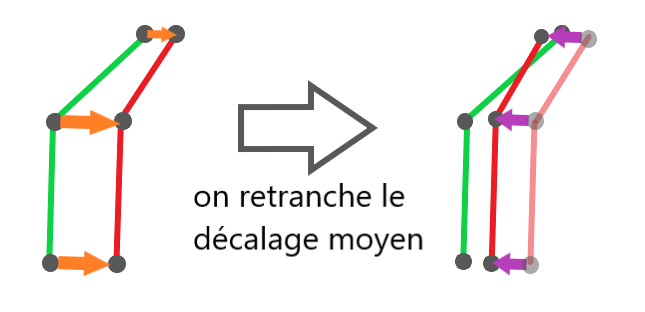
\includegraphics[width=8cm]{offset_sub}
    \end{figure}
    $\bullet \quad$ \underline{Coefficient de proximité} : \newline \newline
    branche $\quad \rightarrow \quad$ suite d'arêtes ordonnées \newline
    Même coefficient que pour les branches
\end{frame}

\subsection{Comparaison}
\begin{frame}{Comparaison de protéines}
    Une fois la plus grande sous-structure isomorphe déterminée : 
    \begin{figure}[!htb]
        \centering
        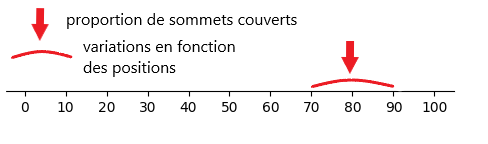
\includegraphics[width=8cm]{0to100}
        \caption{\label{fig:0to100} coefficient de proximité des protéines}
    \end{figure}
\end{frame}

\begin{frame}{Comparaison de protéines}
    \begin{multicols}{2}
        \begin{figure}[!htb]
            \centering
            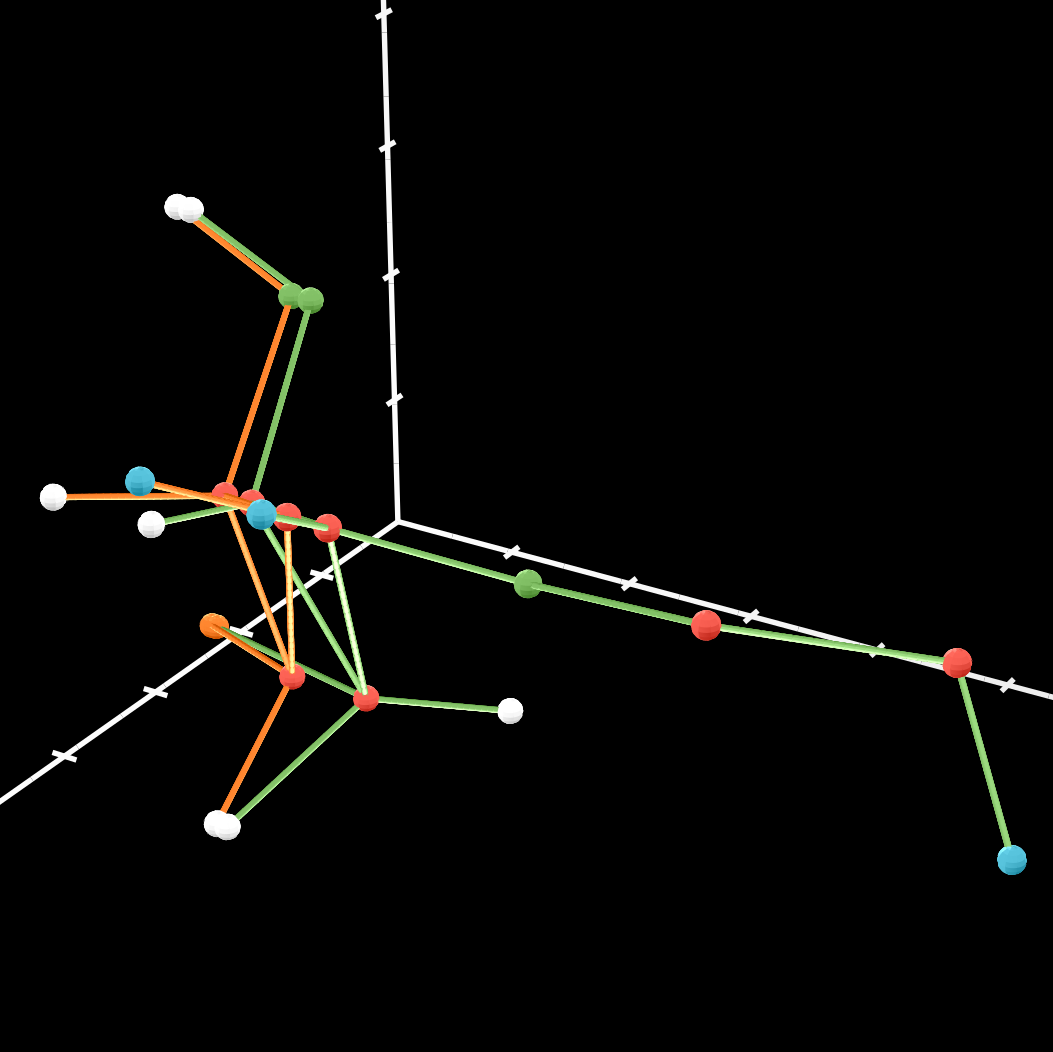
\includegraphics[width = 4cm]{comp_sub_loin}
            \caption{\label{fig: subcomp_loin} Protéines plutôt éloignées}
        \end{figure}
        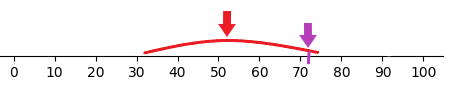
\includegraphics[width = 4cm]{0to100_loin}
        \begin{center}
            $C_{prox}=92.9 \quad C_{struct}=52$\newline \newline
            $\boxed{C=72}$
        \end{center}
    \end{multicols}
    \begin{multicols}{2}
        \begin{figure}[!htb]
            \centering
            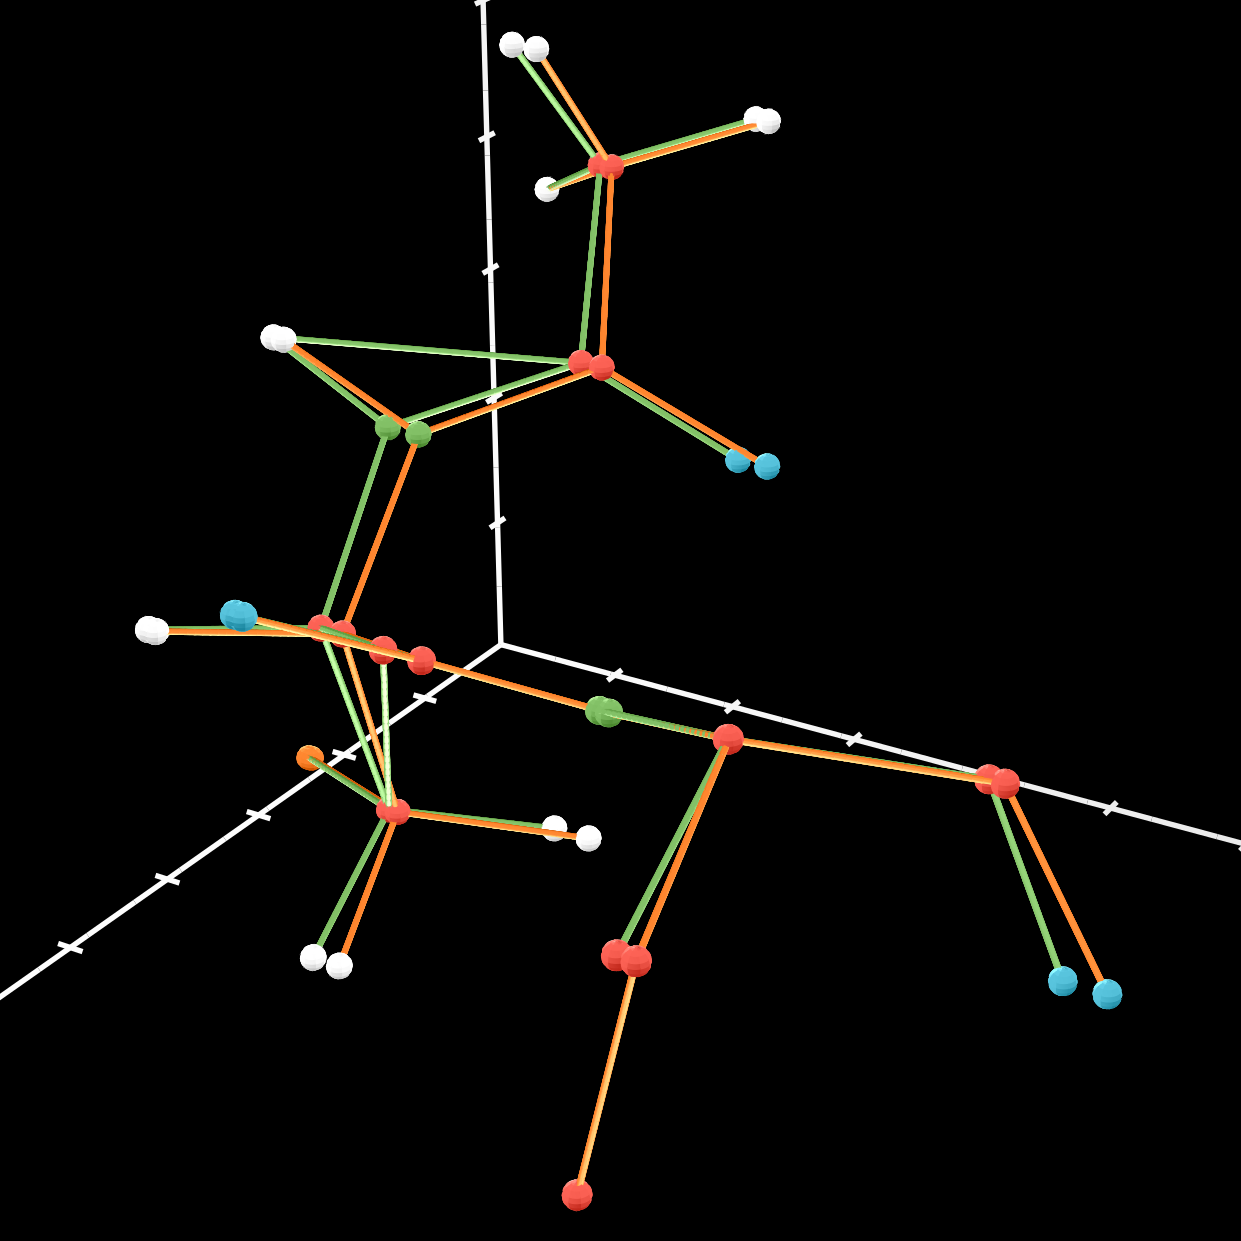
\includegraphics[width = 4cm]{comp_sub_proche}
            \caption{\label{fig: subcom_proche} Protéines plutôt proches}
        \end{figure}
        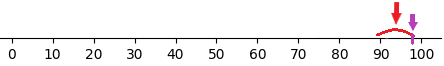
\includegraphics[width=4cm]{0to100_proche}
        \begin{center}
            $C_{prox}=97.7 \quad C_{struct}=93$\newline \newline
            $\boxed{C=96.3}$
        \end{center}
    \end{multicols}
\end{frame}



\section{Conclusion}
\begin{frame}{Conclusion}
    \underline{Bilan} :
    \begin{itemize}
        \item tri des atomes très classant
        \item test d'isomorphisme efficace sur les protéines
        \item méthode recherche du plus grand sous-graphe isomorphe fonctionnelle 
        \item mise en place d'un coefficient de comparaison
    \end{itemize}
    \underline{Limites} : 
    \begin{itemize}
        \item lecture partielle du format pdb
        \item coefficients déterminés de manière empirique
        \newline $\quad \rightarrow \quad$sur une base d'exemples, ajuster les valeurs
        \item recherche demande beaucoup de ressources (NP-complet)
    \end{itemize}
\end{frame}

\section{Annexe}

\part{Annexe}
\begin{frame}[noframenumbering]{Annexe}
\begin{multicols}{2}
\tableofcontents
\end{multicols}
\end{frame}

\section{Annexe Mckay}
\subsection{Arbre de recherche}
\begin{frame}[noframenumbering]{Arbre de recherche de permutations}
    \begin{minipage}{0.3\textwidth}
        \begin{figure}[!htb]
            \centering
            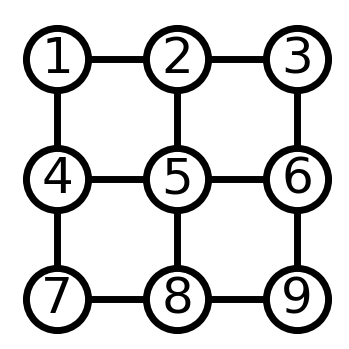
\includegraphics[width = 1.7cm]{graph_tri_equal}
            \caption{\label{fig: Graph G2}Graph G}
        \end{figure}
    \end{minipage}
    \begin{minipage}{0.6\textwidth}
        \begin{center}
            On considère le tri suivant le degré :\newline
            $\pi = (1\ 3\ 7\ 9\ |\ 2\ 4\ 6\ 8\ |\ 5)\qquad $ \newline \newline
            $R(\pi)=\pi$ est alors la racine de l'arbre
        \end{center}
    \end{minipage}
    \newline \newline \newline
    \underline{Trouver les fils} :
    \begin{itemize}
        \item trouver la première partie $V_i$ d'au moins 2 éléments de $\pi$
        \item pour $v \in V$, on crée \textbf{artificiellement} un nouveau tri équitable :
        $\quad \longrightarrow \quad \pi_v = \pi \perp v = R(\ (V_1|..|\ \lbrace v \rbrace \ |\ V_i \textbackslash \lbrace v \rbrace\ |..)\ )$
        \item chacun des tris créés est un fils, on réitère jusqu'à obtenir des tris triviaux (paquets de taille 1)
    \end{itemize}
\end{frame}

\begin{frame}[noframenumbering]{Arbre de recherche de permutations}
    \begin{figure}[!htb]
        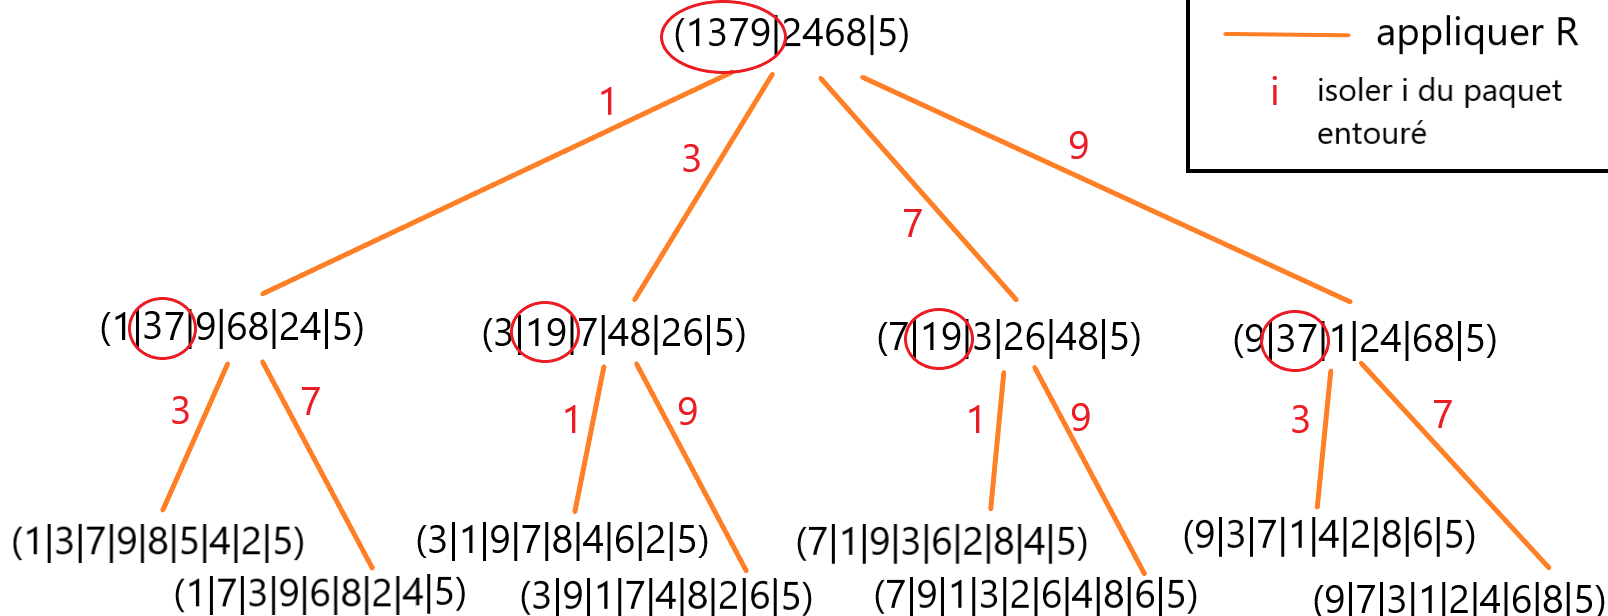
\includegraphics[width = 10cm]{search_tree}
        \caption{\label{fig:Arbre T(G)} Arbre T(G) de racine $\pi=(1\ 3\ 7\ 9\ |\ 2\ 4\ 6\ 8\ |\ 5)$}
    \end{figure}
\end{frame}

\subsection{Isomorphisme cannonique}
\begin{frame}[noframenumbering]{Relation d'ordre sur les graphes et isomorphisme cannonique}
    \underline{Ordre total $\preceq$ sur les graphes} : \newline \newline
    On pose la fonction $i:\ G\ \longmapsto i(G)$ telle que : \newline
    $\quad \bullet \ i(G)$ est la séquence binaire $(\mathds{1}_{(i,j)\in G})$ dans l'ordre lexicographique \newline
    $\quad \bullet \ G \preceq H$ si et seulement si $i(G) \leq i(H)$ en décimal
    \newline \newline
    On pose alors l'\textbf{ismorphisme cannonique de McKay} (pour le tri $\pi$):
    \begin{equation}
        \boxed{C_M(G) = max_{\preceq}\ \lbrace G^{\sigma},\ \sigma \text{ noeud terminal de T(G) de racine } \pi \rbrace }
    \end{equation}
    alors:
    \begin{equation}
        \boxed{G \cong H \text{ si et seulement si } C_M(G) = C_M(H)}
    \end{equation}
    \newline
    \underline{Exemple} : pour $\pi = (1\ |\ 3\ 7\ |\ 9\ |\ 6\ 8\ |\ 2\ 4\ |\ 5)$
    \begin{multicols}{2}
        \begin{figure}[!htb]
            \centering
            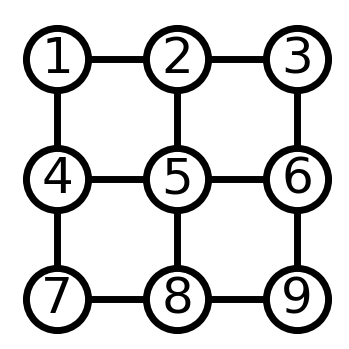
\includegraphics[width = 2.5cm]{graph_tri_equal}
            \caption{\label{fig: Graphe G}Graphe G}
        \end{figure}
        \vspace*{1cm}
        \begin{figure}[!htb]
            \centering
            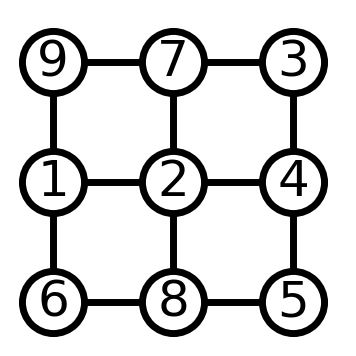
\includegraphics[width = 2.5cm]{cmg}
            \caption{\label{fig: Isomorphe G} Graphe $C_M(G)$}
        \end{figure}
    \end{multicols}
\end{frame}

\begin{frame}[allowframebreaks,noframenumbering]
    \section{Lecture PDB et génération des exemples}
    \subsection{Extraction du fichier PDB}
    \lstinputlisting[lastline=79]{extract_PDB.py}
    \subsection{Génerer les branches}
    \lstinputlisting{generer_nuage.py}
    \subsection{Modifier les protéines}
    \lstinputlisting{generer_protein.py}
    \subsection{Arbre couvrant}
    \lstinputlisting{arbre_couvrant.py}
    \subsection{Générer les graphes}
    \lstinputlisting{creer_graph.py}
    \subsection{Exemples protéines}
    \lstinputlisting[firstline=83]{extract_PDB.py}
\end{frame}
\begin{frame}[allowframebreaks,noframenumbering]
    \section{Définition des classes}  
    \subsection{Branches}
    \lstinputlisting[firstline=1,lastline=124]{cas_simple_nuage.py}
    \subsection{Graphes}
    \lstinputlisting[firstline=1,lastline=37]{graphisomorphism.py}
    \subsection{Protéines}
    \lstinputlisting[firstline=1,lastline=87]{def_protein.py}    
\end{frame}
\begin{frame}[allowframebreaks,noframenumbering]   
    \section{Isomorphisme et sous-isomorphisme}
    \subsection{Isomorphsime sur les graphes}
    \lstinputlisting[firstline=39]{graphisomorphism.py}
    \subsection{Isomorphsime sur les protéines}
    \lstinputlisting[firstline=88]{def_protein.py}
    \subsection{Sous-isomorphisme sur les protéines}
    \lstinputlisting[firstline=14,lastline=68]{subisom_prot.py}
    \subsection{Informations et temps d'exécution}
    \lstinputlisting{isom_prot.py}
    \lstinputlisting[firstline=68,lastline=73]{subisom_prot.py}
\end{frame}
\begin{frame}[allowframebreaks,noframenumbering]
    \section{Fonctions auxiliaires}
    \lstinputlisting{geometrie_et_aux.py}
\end{frame}
\begin{frame}[allowframebreaks,noframenumbering]
    \section{Calcul des coefficients}
    \lstinputlisting[firstline=126,lastline=154]{cas_simple_nuage.py}
    \lstinputlisting[firstline=91]{subisom_prot.py}
\end{frame}
\begin{frame}[allowframebreaks,noframenumbering]
    \section{Affichage}
    \subsection{Graphique complexité}
    \lstinputlisting{plot_graph_complexite_isom_brutes.py}
    \subsection{Affichage branches}
    \lstinputlisting{plot_distlines.py}
    \subsection{Affichage protéines}
    \lstinputlisting{plot_protein.py}
    \subsection{Affichage comparaison protéines}
    \lstinputlisting{plot_sub.py}
\end{frame}

\end{document}


